% !TEX TS-program = pdflatex
% !TEX encoding = UTF-8 Unicode

% This is a simple template for a LaTeX document using the "article" class.
% See "book", "report", "letter" for other types of document.

\documentclass[11pt]{article} % use larger type; default would be 10pt

\usepackage[utf8]{inputenc} % set input encoding (not needed with XeLaTeX)

%%% Examples of Article customizations
% These packages are optional, depending whether you want the features they provide.
% See the LaTeX Companion or other references for full information.

%%% PAGE DIMENSIONS
\usepackage{geometry} % to change the page dimensions
\geometry{a4paper} % or letterpaper (US) or a5paper or....
% \geometry{margin=2in} % for example, change the margins to 2 inches all round
% \geometry{landscape} % set up the page for landscape
%   read geometry.pdf for detailed page layout information

\usepackage{amsmath}
\usepackage{amsthm}
\usepackage{amsfonts}
\usepackage{graphicx} % support the \includegraphics command and options

% tickz includes
\usepackage{tikz}
\usepackage{pgf}
\usepackage{mathrsfs}
\usetikzlibrary{arrows}
% \usepackage[parfill]{parskip} % Activate to begin paragraphs with an empty line rather than an indent

%%% PACKAGES
\usepackage{bbm}
\usepackage{booktabs} % for much better looking tables
\usepackage{array} % for better arrays (eg matrices) in maths
\usepackage{paralist} % very flexible & customisable lists (eg. enumerate/itemize, etc.)
\usepackage{verbatim} % adds environment for commenting out blocks of text & for better verbatim
\usepackage{subfig} % make it possible to include more than one captioned figure/table in a single float
% These packages are all incorporated in the memoir class to one degree or another...
\usepackage{amsthm}
\usepackage{fdsymbol}

%%% HEADERS & FOOTERS
\usepackage{fancyhdr} % This should be set AFTER setting up the page geometry
\pagestyle{fancy} % options: empty , plain , fancy
\renewcommand{\headrulewidth}{0pt} % customise the layout...
\lhead{}\chead{}\rhead{}
\lfoot{}\cfoot{\thepage}\rfoot{}

%%% SECTION TITLE APPEARANCE
\usepackage{sectsty}
\allsectionsfont{\sffamily\mdseries\upshape} % (See the fntguide.pdf for font help)
% (This matches ConTeXt defaults)

%%% ToC (table of contents) APPEARANCE
\usepackage[nottoc,notlof,notlot]{tocbibind} % Put the bibliography in the ToC
\usepackage[titles,subfigure]{tocloft} % Alter the style of the Table of Contents
\renewcommand{\cftsecfont}{\rmfamily\mdseries\upshape}
\renewcommand{\cftsecpagefont}{\rmfamily\mdseries\upshape} % No bold!
\usetikzlibrary{arrows.meta}
\usetikzlibrary{svg.path}
\usetikzlibrary{calc}
%%% END Article customizations

%%% The "real" document content comes below...

\title{Some Presentations of Planar Algebras with Applications to Invariant Theory}
\author{Ryan Vitale}
%\date{} % Activate to display a given date or no date (if empty),
         % otherwise the current date is printed 



%%% Macros

\newcommand{\repz}{Rep$_{K,1}(\mathbb{Z})$}
\newcommand{\h}[2]{\{#1..#2\}}


%\newcommand{\dotmap}{
%\begin{tikzpicture}
%\draw [line width=1.1pt] (0,0) -- (0,1.5ex);
%\draw [fill=black] (0,1.5ex) circle (0.7pt); 
%\end{tikzpicture}
%}

%\newcommand{\lcap}{
%\begin{tikzpicture}
%\draw [line width=1.1pt] (0,0) -- (0,1.75ex);
%\draw [line width=1.1pt] (0,1.75ex) -- (0.5ex,1.75ex);
%\end{tikzpicture}
%}

\newcommand{\lcap}{\boldmath$\langle$\unboldmath}
\newcommand{\rcap}{\boldmath$\rangle$\unboldmath}
\newcommand{\dotmap}{$\bullet$}

%\newcommand{\rcap}{
%\begin{tikzpicture}
%\draw [line width=1.1pt] (0.5ex,0) -- (0.5ex,1.75ex);
%\draw [line width=1.1pt] (0.5ex,1.75ex) -- (0,1.75ex);
%\end{tikzpicture}
%}

\usetikzlibrary{decorations.markings}
\usetikzlibrary{arrows.meta}

\begin{document}

\newtheorem{mydef}{Definition}
\newtheorem{prop}{Proposition}
\newtheorem{lemma}{Lemma}

\maketitle

\section{Introduction}

\section{Background}
\def\marker{$\star$}

An \textbf{oriented planar tangle (OPT)} is a template for combining elements of an \textbf{oriented planar algebra (OPA)}. Input discs and an output disc are connected by oriented strands specifying the type of the inputs and outputs, and a boundary interval is marked (\marker) on each disc to align inputs rotationally. These tangles are defined up to planar isotopy of the strands.
\begin{center}
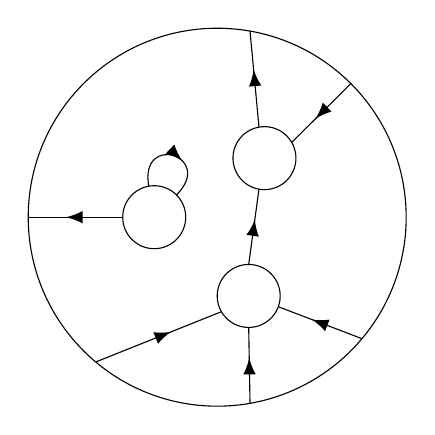
\begin{tikzpicture}
\coordinate (o) at (0,0);
\coordinate (o1) at (0.6,0.75);
\coordinate (o2) at (-0.8,0);
\coordinate (o3) at (0.4,-1);
\def\radout{2.4cm}
\def\radin{0.4cm}
\draw (o) circle[radius=\radout];
\draw (o1) circle[radius=\radin];
\draw (o2) circle[radius=\radin];
\draw (o3) circle[radius=\radin];



\begin{scope}[decoration={
    markings,
    mark=at position 0.6 with {\arrow[scale=1.5]{latex}}}
    ]
\draw [postaction={decorate}] ($ (o) + (45:\radout) $) to ($ (o1) + (30:\radin) $);
\draw [postaction={decorate}] ($ (o1) + (100:\radin) $) to ($ (o) + (80:\radout) $);
\draw [postaction={decorate}] ($ (o3) + (90:\radin) $) to ($ (o1) + (260:\radin) $);
\draw [postaction={decorate}] ($ (o2) + (180:\radin) $) to ($ (o) + (180:\radout) $);
\draw [postaction={decorate}] ($ (o2) + (100:\radin) $) to [controls = +(100:0.7) and +(45:0.7)] ($ (o2) + (45:\radin) $);
\draw [postaction={decorate}] ($ (o) + (280:\radout) $) to ($ (o3) + (270:\radin) $);
\draw [postaction={decorate}] ($ (o) + (320:\radout) $) to ($ (o3) + (340:\radin) $);
\draw [postaction={decorate}] ($ (o) + (230:\radout) $) to ($ (o3) + (210:\radin) $);
\draw ($(o) + (130:\radout-0.2cm) $) node {\marker};
\draw ($(o1) + (-40:\radin+0.2cm) $) node {\marker};
\draw ($(o2) + (140:\radin+0.2cm) $) node {\marker};
\draw ($(o3) + (240:\radin+0.2cm) $) node {\marker};
\end{scope}
\end{tikzpicture}
\end{center}

The space of OPTs form an operad, where composition is performed by inserting some tangle into an input disc of another tangle with each \marker \hspace{1mm}aligned. This composition is defined when the number of strands and their orientations match on the input and output discs.

(picture)
  
An OPA is a collection of vector spaces on which the operad acts. We group elements of an OPA by type into vector spaces $B_\sigma$ called \textbf{box spaces}, indexed by elements $\sigma \in \{+,-\}^n$. The index carries the information of the number of strands $n$, and the orientations of each strand at the disc boundary, ordered counterclockwise from the \marker \hspace{1mm}($+$ for incoming and $-$ for outgoing). We consider oriented Temperley-Lieb as a first example.

\subsection{Oriented Temperley-Lieb, OTL($\delta$)}

Consider the planar algebra of all oriented tangles with no input discs, and where the value of the oriented circle is $\delta$. The box space $B_{(+,-,+,-)}$ is generated as a vector space by the following $2$ tangles.

(picture of tangles)

\subsection{Oriented Symmetric Planar Algebras (OSPA)}
In a symmetric planar algebra we want to allow strand crossings. We make the following alteration to the definition of planar isotopy.
\begin{mydef}
A \textbf{symmetric isotopy} is a planar isotopy allowing the introduction and removal of transverse strand crossings, Reidemeister moves, and naturality (we can pull function nodes across strands).
\end{mydef}

\begin{itemize}
\item picture example of symmetric isotopy
\item example OTL($\delta$) with symmetric structure is OSTL($\delta$)
\end{itemize}

\subsection{Oriented Symmetric Planar Algebras Generated by a Set of Vertices}



\begin{mydef}
Let $S$ be our generating set of vertices, where each vertex has some identifying symbol, and tuples of incoming and outgoing oriented strands called the degrees. The OSPA generated by $S$ is the collection of locally oriented graphs on the vertex set $S$ respecting the degrees of each vertex (i.e. the degrees of each vertex are fixed and part of the data of the vertex). We call a path along any graph a (strand) component. 

%Let $X=(0,1) \times [0,1) \subset \mathbb{R}^2$. Let $U$ be a union of smooth decorated intervals immersed in $X$, whose %endpoints are either at the boundary or at a dot (and not at the same dot or same point on the boundary). These intervals are %locally oriented, and the orientations switch only at brackets. We refer to the connected component of $X-U$ adjacent to
%(0,1) \times \{1\}$ as the \textbf{sky}, and refer to $(0,1) \times \{0\}$ as the \textbf{ground}.
\end{mydef}

\begin{itemize}
\item generic example
\item free OSPA on dots and brackets
\item dual of vertex
\item symmetric and antisymmetric self dual
\item rotational symmetry/eigenvectors
\end{itemize}



\subsection{Disoriented Temperley Lieb, DTL($\delta$)}



\subsection{Pivotal Symmetric Tensor Categories and OSPAs}

Given a pivotal tensor category $C$ and some object $V$ in $C$, we can define an OPA $P(C,V)$. We think of the oriented strands of the planar algebra as being copies of $V$ or $V^*$ for positively or negatively oriented strands respectively. A disjoint union of $n$ oriented strands is then a tensor product of copies of $V$ and $V^*$ with $n$ total factors. Elements of the planar algbera are morphisms in $C$ between tensor products involving $V$ and $V^*$, and the index of the box spaces indicate the domain and target of our maps (e.g. $(+,-,-,+) \mapsto V \otimes V^* \otimes V^* \otimes V$).

(pictures)

Additional structure of $C$ can be reflected in the diagrams of the planar algebra. If $C$ is symmetric we get an OSPA; a strand crossing is then interpreted as a component map of the natural isomorphism defining the symmetric structure. We will be in the case of a symmetric pivotal tensor category, specifically a category of representations of a group.

\subsection{Rep(G,V,k) as an OSPA}
Fix a group $G$, a field $k$, and some object $V\in \text{Rep}_k(G)$, the category of $k$-linear representations of $G$. We study $\text{Alg}(G,V,k)$, the full subcategory of $\text{Rep}_k(G)$ whose objects are finite tensor products of $V$ and $V^{\ast}$. Our goal will be to give a diagrammatic presentation of $\text{Alg}(G,V,k)$, i.e. to give a map of planar algebras $T:\text{Diag}(G,V,k) \rightarrow \text{Alg}(G,V,k)$ for some diagrammatic planar algebra. In all examples considered it will be true that $V \simeq V^{\ast}$, so we can restrict to studying the spaces $\text{Hom}(V^{\otimes n},V^{\otimes m})$. Further, since $\text{Hom}(A, B \otimes C) \simeq \text{Hom}(A\otimes B^{\ast},C)$ for $A,B,C$ finite dimensional representations of a group, we can restrict to studying the spaces $B_n := \text{Hom}(V^{\otimes n}, \mathbbm{1})$.

To construct $\text{Diag}(G,V,k)$ we start with an OSPA generated by some vertex set, and take a quotient to include relations. In defining $T$ we will map an upwards oriented strand to the identity map on $V$ and a downward oriented strand to the identity map on $V^{\ast}$. We have evaluation and coevaluation maps $V^{\ast} \otimes V \xrightarrow{\epsilon} k$, $k \xrightarrow{\eta} V \otimes V^{\ast}$ which will be the image of arcs connecting appropriately oriented strands. We fix an isomorphism $\varphi:V \xrightarrow{\sim} V^{\ast}$ and make this the image under $T$ of the vertex $\varphi$ between an upward and downward oriented strand. (clean these pictures to T(X)=Y form)

\begin{tikzpicture}[scale=0.9]
\clip (-2,2.9) rectangle (16,5.8);
\begin{scope}[decoration={
    markings,
    mark=at position 0.5 with {\arrow[scale=1.25]{latex}}}
    ]
\draw [-,postaction={decorate}] (0,3) to (0,5.5);
\draw (0.5,4.25) node[scale=1.25] {$\xrightarrow{T}$};

\draw [-,postaction={decorate}] (3,5.5) to (3,3);
\draw (3.5,4.25) node[scale=1.25] {$\xrightarrow{T}$};

\draw (1.25,4.05) node {$\text{Id}_V$};
\draw (4.3,4.05) node {$\text{Id}_{V^{\ast}}$};

\draw [-,postaction={decorate}] (7.25,3) to  [controls=+(90:1) and +(90:1)] (5.75,3);

\draw [-,postaction={decorate}] (7.25,5.5) to  [controls=+(-90:1) and +(-90:1)] (5.75,5.5);

\draw (7.8,3.25) node[scale=1.25] {$\xrightarrow{T} \eta$};
\draw (7.8,5) node[scale=1.25] {$\xrightarrow{T} \epsilon$};

\draw (9.55,4) rectangle (10,4.5);
\draw (9.8,4.25) node {$\varphi$};

\draw [-,postaction={decorate}] (9.75,3) to (9.75,4);
\draw [-,postaction={decorate}] (9.75,5.5) to (9.75,4.5);

\draw (10.7,4.35) node[scale=1.25] {$\xrightarrow{T} \varphi$};

\end{scope}
\end{tikzpicture}


Using $\varphi$ along with evaluation we can turn outgoing strands into incoming ones, illustrating the isomorphism $\text{Hom}(V^{\otimes n},V^{\otimes m}) \xrightarrow{\sim} \text{Hom}(V^{\otimes (n+m)}, \mathbbm{1})$, and allowing us to focus on pictures where all strands are `attached to the ground'. (define ground prior to this)

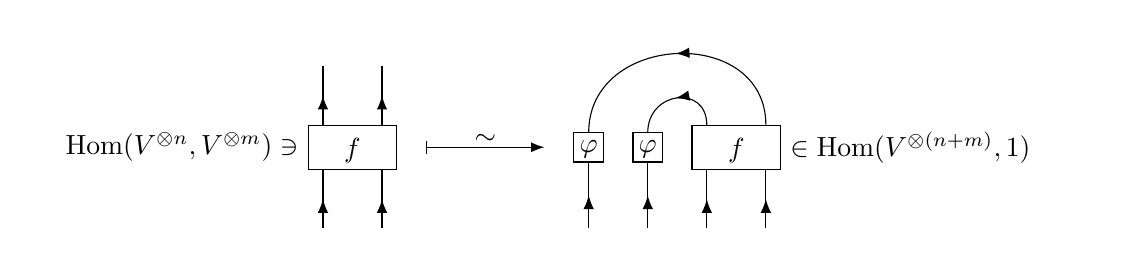
\begin{tikzpicture}[x=0.75cm,y=0.75cm]
\clip (-2.5,-.1) rectangle (16,3.4);
\begin{scope}[decoration={
    markings,
    mark=at position 0.5 with {\arrow[scale=1.25]{latex}}}
    ]

\draw (2.25,1) rectangle (3.75,1.75);
\draw (3, 1.325) node {$f$};

\draw (2.25,1.375) node[anchor=east] {$\text{Hom}(V^{\otimes n}, V^{\otimes m}) \ni $};

\draw [|->,>=Latex] (4.25,1.375) to (6.25,1.375);

\draw (5.25,1.5) node {$\sim$};


\draw (8.75,1) rectangle (10.25,1.75);

\draw (9.5, 1.325) node {$f$};

\draw (6.75,1.125) rectangle (7.25,1.625);
\draw (7.75,1.125) rectangle (8.25,1.625);

\draw (7,1.35) node {$\varphi$};
\draw (8,1.35) node {$\varphi$};

\draw [-,postaction={decorate}] (9,1.75) to [controls=+(90:0.7) and +(90:0.7)] (8,1.625);
\draw [-,postaction={decorate}] (10,1.75) to [controls=+(90:1.7) and +(90:1.7)] (7,1.625);

\foreach \x in {2.5,3.5,9,10}
	\draw [-,postaction={decorate}] (\x,0) to (\x,1);
	
\foreach \x in {7,8}
	\draw [-,postaction={decorate}] (\x,0) to (\x,1.125);

\foreach \x in {2.5,3.5}
	\draw [-,postaction={decorate}] (\x,1.75) to (\x,2.75);

\draw (10.25,1.375) node[anchor=west] {$ \in \text{Hom}(V^{\otimes (n+m)},\mathbbm{1})$};

% cap rhs with varphi isos

\end{scope}
\end{tikzpicture}


\subsection{Outline of Technique for Finding a Diagrammatic Presentation of Rep(G,V,k)}
 Our goal is to determine a minimal generating set of pictures and relations so that the resulting diagrammatic planar algebra, call it $\text{Diag}{(G,V,k)}$, will be isomorphic to $P_{G,V,k}$. In each example we use the following procedure:
 \begin{enumerate}
 \item Define generating pictures and relations for $\text{Diag}{(G,V,k)}$, and give a map of planar algebras $\text{Diag}{(G,V,k)} \xrightarrow{T} P_{G,V,k}$.
 \item For each $n$ find a subset $D_n \subset \text{Diag}{(G,V,k)}$ such that $T(D_n)$ is a basis for $B_n$. Exhibiting such $D_n$ shows that $T$ is surjective, since as argued above $M_{G,V,k}$ is determined by the spaces $B_n$.
 \item Show that an arbitrary picture in $\text{Diag}{(G,V,k)}$ can be rewritten linearly in terms of elements of the $D_n$ using the presented relations. This shows that $T$ is injective, so that $\text{Diag}{(G,V,k)} \simeq P_{G,V,k}$ as planar algebras. 
 
 \end{enumerate}

If we fix coordinates on $V$, when describing the spaces $B_n$ we are also describing a subring of vector invariants for $G$, i.e. each $f$ in $B_n$ is also in $(V^{\oplus n})^G=\{f \in k[x_1,\ldots,x_n] : \forall g \in G, f(\bar{x}) = f(g \cdot \bar{x})\}$. This follows from observing that the defining property for an element of $(V^{\oplus n})^G$ is the same as the defining property for a map of $G$ representations from $V^{\otimes n}$ to the trivial representation. Giving a presentation of $\text{Alg}{(G,V,k)}$ is then related to giving a first and second fundamental theorem of invariant theory for $(V^{\oplus n})^G$, and in each example we discuss this relationship.



\section{A 2-dimensional $\mathbb{Z}$-representation over $\mathbb{C}$}

Let $V_n=(\mathbb{C}^n,\phi_n)$ where $\phi_n: \mathbb{Z} \rightarrow GL(\mathbb{C}^n)$ is defined by $\phi_n(1)=J_n$, and $J_n$ is the Jordan block of dimension $n$ with eigenvalue $1$. In this section we set $V=V_2$ and study $\text{Alg}{(\mathbb{Z},V, \mathbb{C})}$. Taking the standard basis of $\mathbb{C}^2$, $v_0 = (1,0)$ and  $v_1 = (0,1)$, we use the isomorphism $\varphi:V \xrightarrow{\sim} V^{\ast}$ defined by $\varphi(v_0)=v_1^{\ast}$, $\varphi(v_1)=-v_0^{\ast}$. We want to describe the spaces $B_n = \text{Hom}(V^{\otimes n},\mathbbm{1} \simeq V_1)$.

\subsection {Presentation of $\text{Diag}{(\mathbb{Z},V,\mathbb{C})}$ and map into $\text{Alg}{(\mathbb{Z},V,\mathbb{C})}$}

\begin{mydef}
We define $\text{Diag}{(\mathbb{Z},V,\mathbb{C})}$ to be the OSPA quotient $G / E$ for the generating set of vertices $G=\{G_1,G_2,G_3\}$ and relations $E=\{E_1,\dots,E_5\}$ below.
\end{mydef}

\begin{tikzpicture}
\begin{scope}[decoration={
    markings,
    mark=at position 0.5 with {\arrow[scale=1.25]{latex}}}
    ]
\clip (-1,-1.25) rectangle (16,4);

\draw [postaction={decorate}] (0,0) circle (17pt);
\draw (1.2,0) node[scale=1.4] {$=$};
\draw (1.2,.05) node[anchor=south,scale=0.8] {$E_3$};
\draw (1.5,.05) node[anchor=west,scale=1.4] {$2$};
\draw [dotted] (-0.9,-1) rectangle (2.25,1);


\draw [-,postaction=decorate] (9.25,-0.75) to (9.25,0.75);
\draw [-,postaction=decorate] (9.75,-0.75) to (9.75,0.75);
\draw (10.25,0) node[scale=1.2] {$+$};

%\draw (0,3) node[anchor=west] {\textbf{Generators:}};
\draw [-,postaction={decorate}] (0,1.5) to (0,2.75);
\draw [fill=black] (0,2.75) circle (1.5pt);

\draw [-,postaction={decorate}] (8,3.25) to (8,1.5);
\draw (7,2.25) node[scale=1.4] {$=$};
\draw (7,2.3) node[anchor=south,scale=0.8] {$E_1$};

\draw [dotted] (5.5,1.25) rectangle (8.5,3.5);
\end{scope}

\draw (-0.1,2.25) node[anchor=east] {$G_1:$};

\begin{scope}[decoration={
	markings,
	mark=at position 0.5 with {\arrow[scale=1.25,thick]{[}},
	mark=at position 0.25 with {\arrow[scale=1.25]{latex}},
	mark=at position 0.8 with {\arrow[scale=1.25,>=latex]{<}}}
	]

\draw [-,postaction={decorate}] (2,3.25) to (2,1.5);
\draw [-,postaction={decorate}] (3.5,-0.75) to (3.5,0.75);
\draw [-,postaction={decorate}] (5.5,0.75) to (5.5,-0.75);

\draw (4.5,0) node[scale=1.4] {$=$};
\draw (4.5,0.05) node[scale=0.8,anchor=south] {$E_4$};
\draw (5,0) node[scale=1.2] {$-$};
\draw [dotted] (3,-1) rectangle (6,1);

\draw [dotted] (6.5,-1) rectangle (12.25,1);
\end{scope}

\draw (1.9,2.25) node[anchor=east] {$G_2:$};


\begin{scope}[decoration={
	markings,
	mark=at position 0.5 with {\arrow[scale=1.25,thick]{]}},
	mark=at position 0.8 with {\arrow[scale=1.25]{latex}},
	mark=at position 0.25 with {\arrow[scale=1.25,>=latex]{<}}}
	]
\draw [-,postaction={decorate}] (4,3.25) to (4,1.5);

\draw [-,postaction={decorate}] (10,3.25) to (10,1.5);
\draw [fill=black] (10,3.25) circle (1.5pt);
\draw [fill=black] (10,1.5) circle (1.5pt);
\draw (11,2.25) node[scale=1.4] {$=$};
\draw (11,2.3) node[anchor=south,scale=0.8] {$E_2$};
\draw (11.5,2.3) node[scale=1.3,anchor=west] {$0$};
\draw [dotted] (9.5,1.25) rectangle (12.25,3.5);

\end{scope}

\begin{scope}[decoration={markings,
	mark=at position 0.35 with {\arrow[scale=1.25,thick]{]}},
	mark=at position 0.55 with {\arrow[scale=1.25,>=latex]{>}},
	mark=at position 0.2 with {\arrow[scale=1.25,>=latex]{<}}}
	]
\draw [-,postaction=decorate] (12,.75) to [controls= +(-90:0.75) and +(-90:0.75)] (10.75,0.7);
\end{scope}
\begin{scope}[decoration={markings,
	mark=at position 0.35 with {\arrow[scale=1.25,thick]{]}},
	mark=at position 0.55 with {\arrow[scale=1.25,>=latex]{<}},
	mark=at position 0.2 with {\arrow[scale=1.25,>=latex]{>}}}
	]
\draw [-,postaction=decorate] (10.75,-0.75) to [controls= +(90:0.75) and +(90:0.75)] (12,-0.75);
\end{scope}

\begin{scope}[decoration={
	markings,
	mark=at position 0.3 with {\arrow[scale=1.25]{latex}},
	mark=at position 0.8 with {\arrow[scale=1.25]{latex}}}
	]

\draw [-,postaction={decorate}] (6.75,-0.75) to (8,0.75);
\draw [-,postaction={decorate}] (8,-0.75) to (6.75,0.75);	

\end{scope}


%\draw [-,postaction={decoration={markings,mark=at position 0.5 with {\arrow{latex}},mark=at position 0.6 with {\arrow{Latex}}},decorate}] (1,1) to (2,2);

\draw [-,postaction={decoration={markings,mark=at position 0.35 with {\arrow[scale=1.25,thick]{[}},mark=at position 0.65 with {\arrow[scale=1.25,thick]{]}},mark=at position 0.2 with {\arrow[scale=1.25,>=latex]{<}},mark=at position 0.8 with {\arrow[scale=1.25,>=latex]{<}},mark=at position 0.53 with {\arrow[scale=1.25,>=latex]{>}}},decorate}] (6,1.5) to (6,3.25);




\draw (3.9,2.25) node[anchor=east] {$G_3:$};



\draw (8.5,0) node[scale=1.4] {$=$};
\draw (8.5,0.05) node[scale=0.8,anchor=south] {$E_5$};





\end{tikzpicture}


\begin{prop}
There is a map of planar algebras $T:\text{Diag}{(\mathbb{Z},V,\mathbb{C})} \rightarrow \text{Alg}{(\mathbb{Z},V,\mathbb{C})}$ determined by the values $T(G_1)=v_1^{\ast},T(G_2)=\varphi$ and $T(G_3)=\varphi^{-1}$. 
\end{prop}

\begin{proof}
We need to show each of $E_1$ through $E_5$ hold in the image of $T$ so that this map is well defined.

\begin{enumerate}[$E_1$:]
\item $\varphi \cdot \varphi^{-1} = \text{Id}_{V^{\ast}}$
\item $1 \mapsto v_1^{\ast} \mapsto v_0 \mapsto 0$
\item $\epsilon \cdot \tau \cdot \eta(1) = \epsilon \cdot \tau (v_1 \otimes v_1^{\ast} + v_0 \otimes v_0^{\ast})=\epsilon(v_1^{\ast} \otimes v_1 + v_0^{\ast} \otimes v_0) = 2$
\item This follows from taking the dual (rotation) of $G_2$ and a coordinate computation:

\begin{tikzpicture}
\clip (-3,0) rectangle (15,2.5);

\begin{scope}[decoration={
	markings,
	mark=at position 0.5 with {\arrow[scale=1.25,thick]{]}},
	mark=at position 0.8 with {\arrow[scale=1.25,>=latex]{<}},
	mark=at position 0.25 with {\arrow[scale=1.25,>=latex]{>}}}
	]

\draw [-,postaction={decorate}] (1,0) to (1,2);

\draw (1.3,2) node {$*$};

\draw (2,1) node {$=$};

\draw [-,postaction={decorate}] (3.5,0.25) to (3.5,1.75);

\draw (3,0.25) to [controls= +(270:0.3) and +(-90:0.3)] (3.5,0.25);
\draw (3.5,1.75) to [controls= +(90:0.3) and +(90:0.3)] (4,1.75);

\draw (3,2) to (3,0.25);
\draw (4,1.75) to (4,0);

\draw (5,1) node {$=$};

\draw [-,postaction={decorate}] (6,2) to (6,0);

\end{scope}

\end{tikzpicture}

\begin{align*}
(&\text{Id}_{V^{\ast}}\otimes \epsilon)(\text{Id}_{V^\ast} \otimes \varphi \otimes \text{Id}_V)(\tau \cdot \eta \otimes \text{Id}_V)(v_0) & &= \\
(&\text{Id}_{V^{\ast}}\otimes \epsilon)(\text{Id}_{V^\ast} \otimes \varphi \otimes \text{Id}_V)(v_0^{\ast} \otimes v_0 \otimes v_0 + v_1^{\ast} \otimes v_1 \otimes v_0) & &= \\
(&\text{Id}_{V^{\ast}}\otimes \epsilon)(v_0^{\ast} \otimes v_1^{\ast} \otimes v_0 - v_1^{\ast} \otimes v_0^{\ast} \otimes v_0) & &= -v_1^{\ast} \\
\end{align*}
\begin{align*}
(&\text{Id}_{V^{\ast}}\otimes \epsilon)(\text{Id}_{V^\ast} \otimes \varphi \otimes \text{Id}_V)(\tau \cdot \eta \otimes \text{Id}_V)(v_1) & &= \\
(&\text{Id}_{V^{\ast}}\otimes \epsilon)(\text{Id}_{V^\ast} \otimes \varphi \otimes \text{Id}_V)(v_0^{\ast} \otimes v_0 \otimes v_1 + v_1^{\ast} \otimes v_1 \otimes v_1) & &= \\
(&\text{Id}_{V^{\ast}}\otimes \epsilon)(v_0^{\ast} \otimes v_1^{\ast} \otimes v_1 - v_1^{\ast} \otimes v_0^{\ast} \otimes v_1) & &= v_0^{\ast}\\
\end{align*}

\item The second term on the RHS takes the values $v_0 \otimes v_0 \mapsto 0, v_1 \otimes v_1 \mapsto 0, v_0 \otimes v_1 \mapsto v_1 \otimes v_0 - v_0 \otimes v_1, v_1 \otimes v_0 \mapsto v_0 \otimes v_1 - v_1 \otimes v_0$, and adding the identity map gives us the LHS.
\end{enumerate}

\end{proof}

\subsection{Exhibiting bases $D_n$ for each $B_n$}

The indecomposable representations that appear in $\otimes$-powers of $V$ are exhausted by the sequence $V_n$. When $i \geq 2$ we have the rule

\begin{equation} \label{eq1}
V \otimes V_i \simeq V_{i+1} \oplus V_{i-1}
\end{equation}

so that the fusion graph $\Gamma$ for $V$ is

\begin{tikzpicture}
\clip(-0.5,-1.85) rectangle (14,-.25);
\foreach \x in {1,...,7}
	\draw (2*\x-2,-1.1) node[anchor=north] {$V_{\x}$};
\foreach \x in {1,...,6}
	{\draw [->, >=latex] (2*\x-2,-1) to (2*\x-0.1,-1);
	\draw [<-, >=latex] (2*\x-1.9,-1) to (2*\x,-1);}
\draw (12,-1) to (13,-1);

\foreach \x in {0,...,6}
	\draw [fill=black] (2*\x,-1) circle (2pt);
\foreach \x in {1,...,3}
	\draw [fill=black] (13+.25*\x,-1) circle (0.5pt);

\draw [->,>=latex] (12.5,-1) to (12.1,-1);

\end{tikzpicture}

\begin{mydef}
Let $P_n$ be the set of paths of length $n$ on $\Gamma$ based at $V_1$. Label edges directed from $V_i$ to $V_{i+1}$ with $R$, and edges directed from $V_{i}$ to $V_{i-1}$ by $L$. Then we can describe $P_n$ as the set of words $w$ of length $n$ in the alphabet $\{R,L\}$ where no initial segment of $w$ has more $L$s than $R$s.
\end{mydef}

\begin{prop}
$\#(P_n)=dim(B_n)$
\end{prop}

\begin{proof}
  We have $\dim(B_n)=\text{dimHom}(V^{\otimes n},\mathbbm{1})=\text{dimHom} \big( \sum{\alpha_i V_i,\mathbbm{1} \big) }=\sum{\alpha_i \text{dimHom}(V_i,\mathbbm{1})}$. Since dimHom$(V_j, \mathbbm{1}) = 1$ for any indecomposable $V_j$, we get dim$(B_n)=\sum{\alpha_i}$, which is the number of summands of $V^{\otimes n}$. We can see summands of $V^{\otimes n}$ are in bijection with $P_n$ by induction on $n$. Assume we have a direct sum decomposition of $V^{\otimes n}$ and a bijection between summands of $V^{\otimes n}$ and $P_n$. By definition of $\Gamma$ the summands of $V^{\otimes (n+1)}$ will be the indecomposables that are adjacent to the summands of $V^{\otimes n}$, so append the adjacency edge to the path from the bijection at level $n$.
\end{proof}

We will then construct a set of maps in bijection with $P_n$, and show these maps are independent, so that this set forms a basis for $B_n$. We first construct a map from the set of paths to the diagrammatic category.
\begin{mydef}
We define a map $\delta_n :P_n \rightarrow \text{Diag}{(\mathbb{Z},V,\mathbb{C})}$. Identify concatenation in a path word $w$ with composition of diagrams, and identify each letter of the alphabet with a portion of a picture as below, where $\emptyset$ signifies the end of the word.

\begin{tikzpicture}[x=.6cm,y=.6cm]
\clip(-3,-0.5) rectangle (20,5);
\begin{scope}[decoration={
    markings,
    mark=at position 0.5 with {\arrow[scale=1.25]{latex}}}
    ]

\draw [dotted] (1,0) rectangle (5,4);
\draw [-,postaction={decorate}] (1,2) to (5,2);
\draw [-,postaction={decorate}] (1,3) to (5,3);
\draw [fill=black] (3,2.25) circle (0.5pt);
\draw [fill=black] (3,2.50) circle (0.5pt);
\draw [fill=black] (3,2.75) circle (0.5pt);
\draw (3,4) node[anchor=south] {$R$};
\draw [-,postaction={decorate}] (3,0) to [controls = +(270:-1) and +(0:-1)] (5,1.5);


\draw [dotted] (6,0) rectangle (10,4);
\draw [-,postaction={decorate}] (6,2) to (10,2);
\draw [-,postaction={decorate}] (6,3) to (10,3);
\draw [fill=black] (8,2.25) circle (0.5pt);
\draw [fill=black] (8,2.5) circle (0.5pt);
\draw [fill=black] (8,2.75) circle (0.5pt);
\end{scope}
\begin{scope}[decoration={
    markings,
    mark=at position 0.5 with {\arrow[scale=1.25,thick]{]}},
    mark=at position 0.25 with {\arrow[scale=1.25]{latex}},
    mark=at position 0.75 with {\arrow[scale=1.25,>=latex]{<}}}
    ]

\draw [-,postaction={decorate}] (8,0) to [controls = +(270:-1) and +(0:1)] (6,1.5);
\end{scope}
\begin{scope}[decoration={
	markings,
	mark=at position 0.45 with {\arrow[scale=1.25]{latex}}}
	]
\draw (8,4) node[anchor=south] {$L$};

\draw [dotted] (11,0) rectangle (15,4);
\draw (13,4) node[anchor=south] {$\emptyset$};


\draw [-,postaction={decorate}] (11,3) to [bend right] (12,3.5);
\draw [-,postaction={decorate}] (11,2) to [bend right] (12.25,2.5);
\draw [fill=black] (12,3.5) circle (1.5pt);
\draw [fill=black] (12.25,2.5) circle (1.5pt);

\draw [fill=black] (11.5,2.25) circle (0.5pt);
\draw [fill=black] (11.5,2.5) circle (0.5pt);
\draw [fill=black] (11.5,2.75) circle (0.5pt);

\end{scope}
\end{tikzpicture}

The number of horiztonal strands in each picture varies, and is equal to the excess of $R$s to $L$s in the segment prior to the current letter of $w$. To define $\delta_n(w)$ replace each letter of $w$ with its identified picture, and then glue each portion end to end, including the picture for $\emptyset$ at the end (glue dots onto any remaining strands at the end).
\end{mydef}

For example, take $w=RRRLLRL$:

\begin{tikzpicture}[x=1.1cm]
\clip (-1.51,-0.5) rectangle (16,1.7);

\draw [dotted] (0,0) rectangle (8,1.5);
\foreach \x in {1,...,7}
	\draw [dotted] (\x,0) to (\x,1.5);
\draw (-1.5,.75) node[anchor=west] {$\delta_7(w)=$};
\draw (8,.75) node[anchor=west] {$=$};
\foreach \x in {1,2,3,6}
	\draw (-0.5 + \x,0) node[anchor=north] {$R$};
\foreach \x in {4,5,7}
	\draw (-0.5 + \x,0) node[anchor=north] {$L$};

\draw (7.5,0) node[anchor=north] {$\emptyset$};

\begin{scope}[decoration={
    markings,
    mark=at position 0.5 with {\arrow{latex}}}
    ]

\draw [-,postaction={decorate}] (0.5,0) to [controls= +(90:0.5) and +(180:0.3)] (1,0.9);
\draw [-,postaction={decorate}] (1.5,0) to [controls= +(90:0.35) and +(180:0.3)] (2,0.7);
\draw [-,postaction={decorate}] (2.5,0) to [controls= +(90:0.2) and +(180:0.3)] (3,0.5);
\foreach \x in {1,...,6}
	\draw [-,postaction={decorate}] (\x,0.9) to (\x+1,0.9);

\draw [-,postaction={decorate}] (2,0.7) to (3,0.7);
\draw [-,postaction={decorate}] (3,0.7) to (4,0.7);

\draw [-,postaction={decorate}] (5.5,0) to [controls = +(90:0.2) and +(180:0.3)] (6,0.5);

\draw [-,postaction={decorate}] (7,0.9) to [bend right] (7.4,1.2);

\draw [fill=black] (7.4,1.2) circle (1.25pt);

\draw [-,postaction={decorate}] (8.85,0) to (8.85,0.6);
\draw [fill=black] (8.85,0.6) circle (1.25pt);

\end{scope}
\begin{scope}[decoration={
	markings,
	mark=at position 0.5 with {\arrow[thick]{]}},
	mark=at position 0.3 with {\arrow[>=latex]{>}},
	mark=at position 0.8 with {\arrow[>=latex]{<}}}
	]

\draw [-,postaction={decorate}] (6.5,0) to [controls= +(90:0.3) and +(0:0.3)] (6,0.5);
\draw [-,postaction={decorate}] (4.5,0) to [controls= +(90:0.4) and +(0:0.4)] (4,0.7);
\draw [-,postaction={decorate}] (3.5,0) to [controls= +(90:0.3) and +(0:0.3)] (3,0.5);

\end{scope}

\begin{scope}[decoration={
	markings,
	mark=at position 0.75 with {\arrow[thick]{]}},
	mark=at position 0.65 with {\arrow[>=latex]{>}},
	mark=at position 0.9 with {\arrow[>=latex]{<}}}
	]

\draw [-,postaction={decorate}] (10.25,0) to [controls = +(90:0.5) and +(90:0.5)] (9.5,0);
\draw [-,postaction={decorate}] (10.5,0) to [controls = +(90:0.9) and +(90:0.9)] (9.25,0);
\draw [-,postaction={decorate}] (11.5,0) to [controls = +(90:0.5) and +(90:0.5)] (10.75,0);

\end{scope}
\end{tikzpicture}
 

The images of $\delta_n$ form our sequence $D_n$. Composing $\delta_n$ with $T$ we get $T_n:P_n \rightarrow B_n$. We want to show the values of $T_n$ are linearly independent, and will use the following lemma.

\begin{lemma} Let $(S,<)$ be a finite ordered set, and $V$ a vector space. If there are maps $f:S \rightarrow V$ and $g:S \rightarrow V^*$ such that for all $x,y \in S$:
\begin{enumerate}
\item $g(x)(f(x)) \neq 0$
\item $x<y \implies g(x)(f(y))=0$
\end{enumerate}
Then both the values of $f$ and the values of $g$ are linearly independent.
\end{lemma}
\begin{proof}
For simplicity replace $S$ with the ordered set $(1,2,\dots,n)$. Consider the $n \times n$ matrix $A$ defined by $A_{i,j}=g(i)(f(j))$. Condition $(1)$ implies entries on the main diagonal of $A$ are non-zero. Condition $(2)$ implies $A$ is upper triangular, so together $(1)$ and $(2)$ imply $A$ is invertible. Any linear dependence among the rows of $A$ implies a linear dependence among the values of $g$, and a dependence among columns of $A$ implies a dependence among the values of $f$, so we have our result.
\end{proof}
\begin{prop}
The values of $T_n$ are linearly independent. 
\end{prop}
\begin{proof}
As in Lemma 1, let $S$ be $P_n$ with lexicographic order ($R>L$), and let $g$ be $T_n$. To define $f$ assign to each $x \in P_n$ a vector $f(x) \in V^{\otimes n}$ by identifying $R$ with $v_1$, $L$ with $v_0$, and concatenation with $\otimes$ (e.g. $f(RRLRLLRL)=v_1 \otimes v_1 \otimes v_0 \otimes v_1 \otimes v_0 \otimes v_0 \otimes v_1 \otimes v_0)$. 
By construction of the pairing we have $g(x)(f(x))=1$, so condition $1$ of Lemma $1$ holds. To show condition $2$ holds, note that if $x<y$ then
\begin{align*} 
f(y) &= v_1^{\otimes i} \otimes v_1 \otimes u, \hspace{5mm} u \in V^{\otimes (n-(i+1))} \\
f(x) &= v_1^{\otimes i} \otimes v_0 \otimes w, \hspace{5mm} w \in V^{\otimes (n-(i+1))}
\end{align*}
so that $g(x)(f(y))$ will have the form

\begin{tikzpicture}[x=1.1cm,y=0.9cm]
\clip (-3,-1) rectangle (10,2.5);
\draw (1,1) rectangle (5,2);
\draw (3,1.5) node {$h$};
\begin{scope}[decoration={
	markings,
	mark=at position 0.5 with {\arrow[>=latex]{>}}}
	]
\foreach \x in {1.25,2,4,4.75}
	\draw [-,postaction=decorate] (\x,0) to (\x,1);
\end{scope}
	
\draw (1.65,0.5) node {$\cdots$};
\draw (4.425,0.5) node {$\cdots$};

\begin{scope}[decoration={
	markings,
	mark=at position 0.8 with {\arrow[thick]{]}},
	mark=at position 0.7 with {\arrow[>=latex]{>}},
	mark=at position 0.9 with {\arrow[>=latex]{<}}}
	]

\draw [-,postaction={decorate}] (3.5,0) to [controls= +(90:0.9) and +(90:0.9)] (2.5,0);
\end{scope}

\draw (3.5,-0.25) node {$v_1$};
\draw (2.5,-0.25) node {$v_1$};

\draw (1.65,0) node[anchor=north] {$\underbrace{v_1 \cdots v_1}_{i-1}$};
\draw (4.37,0) node[anchor=north] {$\underbrace{\hspace{4mm}u \hspace{4mm}}_{n-(i+1)}$};

\end{tikzpicture}
which vanishes since looking at the value of the map on positions $i$ and $i+1$,  $(\epsilon)(-\varphi \otimes \text{Id}_{V})(v_1 \otimes v_1)=\epsilon(v_0^{\ast} \otimes v_1)=0$.
\end{proof}

 We then have a basis for each $B_n$ described as images of a set of diagrams $D_n \subset \text{Diag}{(\mathbb{Z},V,\mathbb{C})}$ under the map $T$.

\subsection{Showing $D_n$ spans $\text{Diag}_n(\mathbb{Z},V,\mathbb{C})$.}

Let $\text{Diag}_n(\mathbb{Z},V,\mathbb{C})$ be the box space of $n$ positively oriented strands. We need to give a description of the pictures in $D_n$, and show that if we take an arbitrary picture in $\text{Diag}_n(\mathbb{Z},V,\mathbb{C})$ we can reduce it to the span of $D_n$.

\begin{mydef} We consider $U \in \text{Diag}_n(\mathbb{Z},V,\mathbb{C})$ to be a member of $D_n$ if:
\begin{enumerate}
\item There are no crossings in $U$.
\item For every dot, there is a path from that dot to the sky which does not intersect $U$.
\item Any strand component in $U$ has at most $1$ vertex.
\item Any bracket is directed towards the leftmost endpoint of a strand component.
\end{enumerate}
\end{mydef}

\begin{prop}
$D_n$ spans $\text{Diag}_n({\mathbb{Z},V,\mathbb{C}})$.
\end{prop}
\begin{proof}
We perform the following algorithm to reduce an arbitrary picture to $D_n$:
\begin{enumerate}
\item Pull all dots to the sky via symmetric isotopy.
\item Use relation $E_5$ (crossing resolution) to remove all crossings.
\item Use $E_1$ (bracket cancellation) and $E_4$ (bracket reversal) to reduce the number of brackets on any path to at most $1$, and to direct any bracket towards the leftmost endpoint (if it has one) of its strand component.
\item Use $E_2$ (dot pair removal) to remove any floating double dots. 
\item Use $E_3$ (circle removal) to remove any floating circles.
\end{enumerate}
After steps $1$ and $2$ have been performed, there will be no crossings and all dots will touch the sky. Steps $3$ through $5$ will not change these properties as they cannot intoduce any new dots or crossings. In step 3 we use bracket cancellation and reversal as necessary to remove the number of brackets to $1$ in the odd case or $0$ in the even case on any component. If a component has two dots on it, it will be oriented outward at both ends and so must have an odd number of brackets and hence only one bracket. Similarly if a component is a closed loop, then in order for it to be consistently oriented there must be an even number of brackets, hence zero brackets.  Bracket reduction is done only at the cost of a sign so that it effects no previous steps. At this point we must be left with a diagram that meets items $1$ through $3$ of Definition $4$, and possibly has some oriented circles and dot pairs which don't meet the boundary. Steps $4$ and $5$ remove these circles at the cost of a constant, and our diagram has been reduced to $D_n$.

.
\end{proof}

We illustrate the algorithm and definition with the example 
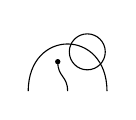
\begin{tikzpicture}[scale=0.5]
\draw [-] (6,18) to [controls = +(90:0.4) and +(-90:0.4)] (5.75,18.75);
\draw [-] (5,18) to [controls = +(90:1.6) and +(90:1.6)] (7,18);
\draw [-] (6.5,19) circle (13pt); 
\draw [fill=black] (5.75,18.75) circle (1.5pt);
\end{tikzpicture}. The leaves of the tree below give all terms which appear in the reduction of our initial diagram.
%\begin{tikzpicture}
%\draw [color=lightgray, fill=lightgray] (0,0) rectangle (8,4);
%\draw [fill=white] (1.7,0) to [controls = +(90:1.25) and +(90:1.5)] (2.5,1.2) to [controls = +(-90:1) and +(90:1.5)] (3,0);
%\draw [fill=white] (4,0) to [controls = +(90:1) and +(150:1)] (4,2.25) to [controls = +(-30:1) and +(225:0.75)] (6,3) to [controls= +(45:1) and %+(50:1)] (6.5,2) to [controls = +(-130:1) and +(90:1)] (7,0);
%\draw [-] (1,0) to [controls = +(90:4.5) and +(-110:4.5)] (1.5,2.25);
%\draw [fill=black] (1.5,2.25) circle (1.5pt);


%\draw [-] (0,0) to (8,0);
%\end{tikzpicture}

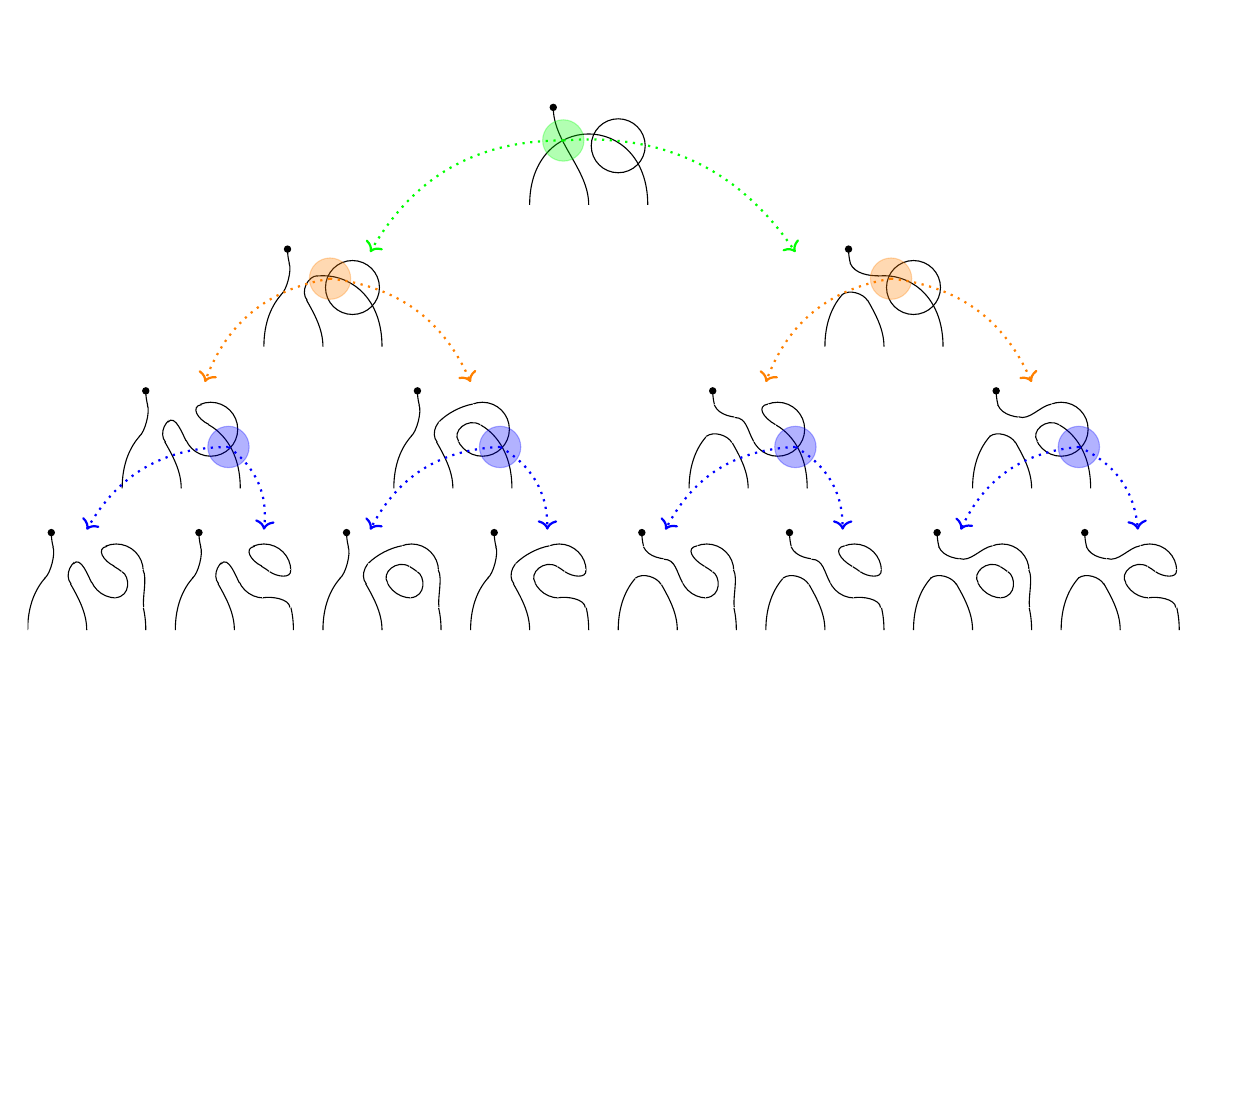
\begin{tikzpicture}[scale = 0.75]
\def\rad{0.35cm}
\def\x0{1.5};
\clip (-2,0) rectangle (18,18);
\draw [-] (6+\x0,15) to [controls = +(90:0.6) and +(-90:0.6)] (5.4+\x0,16.65);
\draw [-] (5+\x0,15) to [controls = +(90:1.6) and +(90:1.6)] (7+\x0,15);
\draw [-] (6.5+\x0,16) circle (13pt); 
\draw [fill=black] (5.4+\x0,16.65) circle (1.5pt);
\draw [color=green,fill=green,opacity=0.3] (5.57+\x0,16.09) circle [radius=\rad];

\draw [->,dotted,color=green,thick] (5.57+\x0,16.09) to [bend right] (3.8,14.2);
\draw [->,dotted,color=green,thick] (5.57+\x0,16.09) to [bend left] (11,14.2);
%%%%%%%%%%%%%%%%%%%%%%%%% lvl 1

\def\x1{-3};
\def\y1{-2.4};

\draw [-] (6+\x1,15+\y1) to [controls = +(90:0.6) and +(-90:0.6)] (5.4+\x1,16.65+\y1);
\draw [-] (5+\x1,15+\y1) to [controls = +(90:1.6) and +(90:1.6)] (7+\x1,15+\y1);
\draw [-] (6.5+\x1,16+\y1) circle (13pt); 
\draw [fill=black] (5.4+\x1,16.65+\y1) circle (1.5pt);
\draw [color=white,fill=white] (5.57+\x1,16.09+\y1) circle [radius=\rad-0.02cm];
\draw [-] ($ (5.57+\x1,16.09+\y1) + (217:\rad) $) to [controls = +(37:0.12) and +(-66:0.12)] ($ (5.57+\x1,16.09+\y1) + (114:\rad) $);
\draw [-] ($ (5.57+\x1,16.09+\y1) + (-62:\rad) $) to [controls = +(130:0.2) and +(180:0.15)] ($ (5.57+\x1,16.09+\y1) + (18:\rad) $);
\draw [color=orange,fill=orange,opacity=0.3] (6.12+\x1,16.15+\y1) circle [radius=\rad];
\draw [->,dotted,color=orange,thick] (6.12+\x1,16.15+\y1) to [bend right] (1,12);
\draw [->,dotted,color=orange,thick] (6.12+\x1,16.15+\y1) to [bend left] (5.5,12);


\def\x2{6.5};
\def\y2{-2.4};

\draw [-] (6+\x2,15+\y2) to [controls = +(90:0.6) and +(-90:0.6)] (5.4+\x2,16.65+\y2);
\draw [-] (5+\x2,15+\y2) to [controls = +(90:1.6) and +(90:1.6)] (7+\x2,15+\y2);
\draw [-] (6.5+\x2,16+\y2) circle (13pt); 
\draw [fill=black] (5.4+\x2,16.65+\y2) circle (1.5pt);
\draw [color=white,fill=white] (5.57+\x2,16.09+\y2) circle [radius=\rad-0.02cm];
\draw [-] ($ (5.57+\x2,16.09+\y2) + (217:\rad) $) to [controls = +(37:0.16) and +(120:0.14)] ($ (5.57+\x2,16.09+\y2) + (-64:\rad) $);
\draw [-] ($ (5.57+\x2,16.09+\y2) + (114:\rad) $) to [controls = +(-66:0.2) and +(180:0.15)] ($ (5.57+\x2,16.09+\y2) + (18:\rad) $);
\draw [color=orange,fill=orange,opacity=0.3] (6.12+\x2,16.15+\y2) circle [radius=\rad];
\draw [->,dotted,color=orange,thick] (6.12+\x2,16.15+\y2) to [bend right] (10.5,12);
\draw [->,dotted,color=orange,thick] (6.12+\x2,16.15+\y2) to [bend left] (15,12);

%%%%%%%%%%%%%%%%%%%%%%%%%% lvl 2

\def\x3{-5.4};
\def\y3{-4.8};

\draw [-] (6+\x3,15+\y3) to [controls = +(90:0.6) and +(-90:0.6)] (5.4+\x3,16.65+\y3);
\draw [-] (5+\x3,15+\y3) to [controls = +(90:1.6) and +(90:1.6)] (7+\x3,15+\y3);
\draw [-] (6.5+\x3,16+\y3) circle (13pt); 
\draw [fill=black] (5.4+\x3,16.65+\y3) circle (1.5pt);
\draw [color=white,fill=white] (5.57+\x3,16.09+\y3) circle [radius=\rad-0.02cm];
\draw [-] ($ (5.57+\x3,16.09+\y3) + (217:\rad) $) to [controls = +(37:0.12) and +(-66:0.12)] ($ (5.57+\x3,16.09+\y3) + (114:\rad) $);
\draw [-] ($ (5.57+\x3,16.09+\y3) + (-62:\rad) $) to [controls = +(130:0.2) and +(180:0.15)] ($ (5.57+\x3,16.09+\y3) + (18:\rad) $);
\draw [color=white,fill=white] (6.12+\x3,16.15+\y3) circle [radius=\rad-0.02cm];
\draw [color=blue,fill=blue,opacity=0.3] (6.8+\x3,15.7+\y3) circle [radius=\rad];
\draw [-] ($ (6.12+\x3,16.15+\y3) + (185:\rad) $) to [controls = +(50:0.2) and +(120:0.1)] ($ (6.12+\x3,16.15+\y3) + (-96:\rad) $);
\draw [-] ($ (6.12+\x3,16.15+\y3) + (50:\rad) $) to [controls = +(190:0.2) and +(155:0.2)] ($ (6.12+\x3,16.15+\y3) + (-11:\rad) $);
\draw [->,dotted,color=blue,thick] (6.8+\x3,15.7+\y3) to [bend right] (-1,9.5);
\draw [->,dotted,color=blue,thick] (6.8+\x3,15.7+\y3) to [bend left] (2,9.5);

\def\x4{-0.8};
\def\y4{-4.8};

\draw [-] (6+\x4,15+\y4) to [controls = +(90:0.6) and +(-90:0.6)] (5.4+\x4,16.65+\y4);
\draw [-] (5+\x4,15+\y4) to [controls = +(90:1.6) and +(90:1.6)] (7+\x4,15+\y4);
\draw [-] (6.5+\x4,16+\y4) circle (13pt); 
\draw [fill=black] (5.4+\x4,16.65+\y4) circle (1.5pt);
\draw [color=white,fill=white] (5.57+\x4,16.09+\y4) circle [radius=\rad-0.02cm];
\draw [-] ($ (5.57+\x4,16.09+\y4) + (217:\rad) $) to [controls = +(37:0.12) and +(-66:0.12)] ($ (5.57+\x4,16.09+\y4) + (114:\rad) $);
\draw [-] ($ (5.57+\x4,16.09+\y4) + (-62:\rad) $) to [controls = +(130:0.2) and +(180:0.15)] ($ (5.57+\x4,16.09+\y4) + (18:\rad) $);
\draw [color=white,fill=white] (6.12+\x4,16.15+\y4) circle [radius=\rad];
\draw [color=blue,fill=blue,opacity=0.3] (6.8+\x4,15.7+\y4) circle [radius=\rad];
\draw [-] ($ (6.12+\x4,16.15+\y4) + (183:\rad) $) to [controls = +(45:0.2) and +(190:0.2)] ($ (6.12+\x4,16.15+\y4) + (52:\rad) $);
\draw [-] ($ (6.12+\x4,16.15+\y4) + (-94:\rad) $) to [controls = +(125:0.2) and +(150:0.25)] ($ (6.12+\x4,16.15+\y4) + (-12:\rad) $);
\draw [->,dotted,color=blue,thick] (6.8+\x4,15.7+\y4) to [bend right] (3.8,9.5);
\draw [->,dotted,color=blue,thick] (6.8+\x4,15.7+\y4) to [bend left] (6.8,9.5);


\def\x5{4.2};
\def\y5{-4.8};

\draw [-] (6+\x5,15+\y5) to [controls = +(90:0.6) and +(-90:0.6)] (5.4+\x5,16.65+\y5);
\draw [-] (5+\x5,15+\y5) to [controls = +(90:1.6) and +(90:1.6)] (7+\x5,15+\y5);
\draw [-] (6.5+\x5,16+\y5) circle (13pt); 
\draw [fill=black] (5.4+\x5,16.65+\y5) circle (1.5pt);
\draw [color=white,fill=white] (5.57+\x5,16.09+\y5) circle [radius=\rad];
\draw [-] ($ (5.57+\x5,16.09+\y5) + (217:\rad) $) to [controls = +(37:0.16) and +(120:0.14)] ($ (5.57+\x5,16.09+\y5) + (-64:\rad) $);
\draw [-] ($ (5.57+\x5,16.09+\y5) + (114:\rad) $) to [controls = +(-66:0.2) and +(180:0.15)] ($ (5.57+\x5,16.09+\y5) + (18:\rad) $);
\draw [color=white,fill=white] (6.12+\x5,16.15+\y5) circle [radius=\rad];
\draw [color=blue,fill=blue,opacity=0.3] (6.8+\x5,15.7+\y5) circle [radius=\rad];
\draw [-] ($ (6.12+\x5,16.15+\y5) + (172:\rad) $) to [controls = +(0:0.2) and +(120:0.2)] ($ (6.12+\x5,16.15+\y5) + (-95:\rad) $);
\draw [-] ($ (6.12+\x5,16.15+\y5) + (52:\rad) $) to [controls = +(190:0.2) and +(150:0.25)] ($ (6.12+\x5,16.15+\y5) + (-12:\rad) $);
\draw [->,dotted,color=blue,thick] (6.8+\x5,15.7+\y5) to [bend right] (8.8,9.5);
\draw [->,dotted,color=blue,thick] (6.8+\x5,15.7+\y5) to [bend left] (11.8,9.5);

\def\x6{9};
\def\y6{-4.8};

\draw [-] (6+\x6,15+\y6) to [controls = +(90:0.6) and +(-90:0.6)] (5.4+\x6,16.65+\y6);
\draw [-] (5+\x6,15+\y6) to [controls = +(90:1.6) and +(90:1.6)] (7+\x6,15+\y6);
\draw [-] (6.5+\x6,16+\y6) circle (13pt); 
\draw [fill=black] (5.4+\x6,16.65+\y6) circle (1.5pt);
\draw [color=white,fill=white] (5.57+\x6,16.09+\y6) circle [radius=\rad-0.02cm];
\draw [-] ($ (5.57+\x6,16.09+\y6) + (217:\rad) $) to [controls = +(37:0.16) and +(120:0.14)] ($ (5.57+\x6,16.09+\y6) + (-64:\rad) $);
\draw [-] ($ (5.57+\x6,16.09+\y6) + (114:\rad) $) to [controls = +(-66:0.2) and +(180:0.15)] ($ (5.57+\x6,16.09+\y6) + (18:\rad) $);
\draw [color=white,fill=white] (6.12+\x6,16.15+\y6) circle [radius=\rad];
\draw [color=blue,fill=blue,opacity=0.3] (6.8+\x6,15.7+\y6) circle [radius=\rad];
\draw [-] ($ (6.12+\x6,16.15+\y6) + (170:\rad) $) to [controls = +(-20:0.2) and +(190:0.2)] ($ (6.12+\x6,16.15+\y6) + (52:\rad) $);
\draw [-] ($ (6.12+\x6,16.15+\y6) + (-94:\rad) $) to [controls = +(125:0.2) and +(150:0.25)] ($ (6.12+\x6,16.15+\y6) + (-12:\rad) $);
\draw [->,dotted,color=blue,thick] (6.8+\x6,15.7+\y6) to [bend right] (13.8,9.5);
\draw [->,dotted,color=blue,thick] (6.8+\x6,15.7+\y6) to [bend left] (16.8,9.5);

%%%%%%%%%%%%%%%%%%%%%%%%%%%% lvl 3

\def\x7{-7};
\def\y7{-7.2};

\draw [-] (6+\x7,15+\y7) to [controls = +(90:0.6) and +(-90:0.6)] (5.4+\x7,16.65+\y7);
\draw [-] (5+\x7,15+\y7) to [controls = +(90:1.6) and +(90:1.6)] (7+\x7,15+\y7);
\draw [-] (6.5+\x7,16+\y7) circle (13pt); 
\draw [fill=black] (5.4+\x7,16.65+\y7) circle (1.5pt);
\draw [color=white,fill=white] (5.57+\x7,16.09+\y7) circle [radius=\rad-0.02cm];
\draw [-] ($ (5.57+\x7,16.09+\y7) + (217:\rad) $) to [controls = +(37:0.12) and +(-66:0.12)] ($ (5.57+\x7,16.09+\y7) + (114:\rad) $);
\draw [-] ($ (5.57+\x7,16.09+\y7) + (-62:\rad) $) to [controls = +(130:0.2) and +(180:0.15)] ($ (5.57+\x7,16.09+\y7) + (18:\rad) $);
\draw [color=white,fill=white] (6.12+\x7,16.15+\y7) circle [radius=\rad-0.02cm];
\draw [color=white,fill=white] (6.8+\x7,15.7+\y7) circle [radius=\rad];
\draw [-] ($ (6.12+\x7,16.15+\y7) + (185:\rad) $) to [controls = +(50:0.2) and +(120:0.1)] ($ (6.12+\x7,16.15+\y7) + (-96:\rad) $);
\draw [-] ($ (6.12+\x7,16.15+\y7) + (50:\rad) $) to [controls = +(190:0.2) and +(155:0.2)] ($ (6.12+\x7,16.15+\y7) + (-11:\rad) $);
\draw [-] ($ (6.8+\x7,15.7+\y7) + (125:\rad) $) to [controls = +(-30:0.15) and +(5:0.27)] ($ (6.8+\x7,15.7+\y7) + (206:\rad) $);
\draw [-] ($ (6.8+\x7,15.7+\y7) + (64:\rad) $) to [controls = +(-60:0.15) and +(100:0.15)] ($ (6.8+\x7,15.7+\y7) + (-62:\rad) $);



\def\x8{-4.5};
\def\y8{-7.2};

\draw [-] (6+\x8,15+\y8) to [controls = +(90:0.6) and +(-90:0.6)] (5.4+\x8,16.65+\y8);
\draw [-] (5+\x8,15+\y8) to [controls = +(90:1.6) and +(90:1.6)] (7+\x8,15+\y8);
\draw [-] (6.5+\x8,16+\y8) circle (13pt); 
\draw [fill=black] (5.4+\x8,16.65+\y8) circle (1.5pt);
\draw [color=white,fill=white] (5.57+\x8,16.09+\y8) circle [radius=\rad-0.02cm];
\draw [-] ($ (5.57+\x8,16.09+\y8) + (217:\rad) $) to [controls = +(37:0.12) and +(-66:0.12)] ($ (5.57+\x8,16.09+\y8) + (114:\rad) $);
\draw [-] ($ (5.57+\x8,16.09+\y8) + (-62:\rad) $) to [controls = +(130:0.2) and +(180:0.15)] ($ (5.57+\x8,16.09+\y8) + (18:\rad) $);
\draw [color=white,fill=white] (6.12+\x8,16.15+\y8) circle [radius=\rad-0.02cm];
\draw [color=white,fill=white] (6.8+\x8,15.7+\y8) circle [radius=\rad];
\draw [-] ($ (6.12+\x8,16.15+\y8) + (185:\rad) $) to [controls = +(50:0.2) and +(120:0.1)] ($ (6.12+\x8,16.15+\y8) + (-96:\rad) $);
\draw [-] ($ (6.12+\x8,16.15+\y8) + (50:\rad) $) to [controls = +(190:0.2) and +(155:0.2)] ($ (6.12+\x8,16.15+\y8) + (-11:\rad) $);
\draw [-] ($ (6.8+\x8,15.7+\y8) + (125:\rad) $) to [controls = +(-35:0.15) and +(-85:0.15)] ($ (6.8+\x8,15.7+\y8) + (64:\rad) $);
\draw [-] ($ (6.8+\x8,15.7+\y8) + (206:\rad) $) to [controls = +(10:0.15) and +(95:0.15)] ($ (6.8+\x8,15.7+\y8) + (-66:\rad) $);


\def\x9{-2};
\def\y9{-7.2};

\draw [-] (6+\x9,15+\y9) to [controls = +(90:0.6) and +(-90:0.6)] (5.4+\x9,16.65+\y9);
\draw [-] (5+\x9,15+\y9) to [controls = +(90:1.6) and +(90:1.6)] (7+\x9,15+\y9);
\draw [-] (6.5+\x9,16+\y9) circle (13pt); 
\draw [fill=black] (5.4+\x9,16.65+\y9) circle (1.5pt);
\draw [color=white,fill=white] (5.57+\x9,16.09+\y9) circle [radius=\rad-0.02cm];
\draw [-] ($ (5.57+\x9,16.09+\y9) + (217:\rad) $) to [controls = +(37:0.12) and +(-66:0.12)] ($ (5.57+\x9,16.09+\y9) + (114:\rad) $);
\draw [-] ($ (5.57+\x9,16.09+\y9) + (-62:\rad) $) to [controls = +(130:0.2) and +(180:0.15)] ($ (5.57+\x9,16.09+\y9) + (18:\rad) $);
\draw [color=white,fill=white] (6.12+\x9,16.15+\y9) circle [radius=\rad];
\draw [color=white,fill=white] (6.8+\x9,15.7+\y9) circle [radius=\rad];
\draw [-] ($ (6.12+\x9,16.15+\y9) + (183:\rad) $) to [controls = +(45:0.2) and +(190:0.2)] ($ (6.12+\x9,16.15+\y9) + (52:\rad) $);
\draw [-] ($ (6.12+\x9,16.15+\y9) + (-94:\rad) $) to [controls = +(125:0.2) and +(150:0.25)] ($ (6.12+\x9,16.15+\y9) + (-12:\rad) $);
\draw [-] ($ (6.8+\x9,15.7+\y9) + (125:\rad) $) to [controls = +(-30:0.15) and +(5:0.27)] ($ (6.8+\x9,15.7+\y9) + (206:\rad) $);
\draw [-] ($ (6.8+\x9,15.7+\y9) + (64:\rad) $) to [controls = +(-60:0.15) and +(100:0.15)] ($ (6.8+\x9,15.7+\y9) + (-62:\rad) $);

\def\x10{0.5};
\def\y10{-7.2};

\draw [-] (6+\x10,15+\y10) to [controls = +(90:0.6) and +(-90:0.6)] (5.4+\x10,16.65+\y10);
\draw [-] (5+\x10,15+\y10) to [controls = +(90:1.6) and +(90:1.6)] (7+\x10,15+\y10);
\draw [-] (6.5+\x10,16+\y10) circle (13pt); 
\draw [fill=black] (5.4+\x10,16.65+\y10) circle (1.5pt);
\draw [color=white,fill=white] (5.57+\x10,16.09+\y10) circle [radius=\rad-0.02cm];
\draw [-] ($ (5.57+\x10,16.09+\y10) + (217:\rad) $) to [controls = +(37:0.12) and +(-66:0.12)] ($ (5.57+\x10,16.09+\y10) + (114:\rad) $);
\draw [-] ($ (5.57+\x10,16.09+\y10) + (-62:\rad) $) to [controls = +(130:0.2) and +(180:0.15)] ($ (5.57+\x10,16.09+\y10) + (18:\rad) $);
\draw [color=white,fill=white] (6.12+\x10,16.15+\y10) circle [radius=\rad];
\draw [color=white,fill=white] (6.8+\x10,15.7+\y10) circle [radius=\rad];
\draw [-] ($ (6.12+\x10,16.15+\y10) + (183:\rad) $) to [controls = +(45:0.2) and +(190:0.2)] ($ (6.12+\x10,16.15+\y10) + (52:\rad) $);
\draw [-] ($ (6.12+\x10,16.15+\y10) + (-94:\rad) $) to [controls = +(125:0.2) and +(150:0.25)] ($ (6.12+\x10,16.15+\y10) + (-12:\rad) $);
\draw [-] ($ (6.8+\x10,15.7+\y10) + (125:\rad) $) to [controls = +(-35:0.15) and +(-85:0.15)] ($ (6.8+\x10,15.7+\y10) + (64:\rad) $);
\draw [-] ($ (6.8+\x10,15.7+\y10) + (206:\rad) $) to [controls = +(10:0.15) and +(95:0.15)] ($ (6.8+\x10,15.7+\y10) + (-66:\rad) $);

\def\x11{3};
\def\y11{-7.2};

\draw [-] (6+\x11,15+\y11) to [controls = +(90:0.6) and +(-90:0.6)] (5.4+\x11,16.65+\y11);
\draw [-] (5+\x11,15+\y11) to [controls = +(90:1.6) and +(90:1.6)] (7+\x11,15+\y11);
\draw [-] (6.5+\x11,16+\y11) circle (13pt); 
\draw [fill=black] (5.4+\x11,16.65+\y11) circle (1.5pt);
\draw [color=white,fill=white] (5.57+\x11,16.09+\y11) circle [radius=\rad];
\draw [-] ($ (5.57+\x11,16.09+\y11) + (217:\rad) $) to [controls = +(37:0.16) and +(120:0.14)] ($ (5.57+\x11,16.09+\y11) + (-64:\rad) $);
\draw [-] ($ (5.57+\x11,16.09+\y11) + (114:\rad) $) to [controls = +(-66:0.2) and +(180:0.15)] ($ (5.57+\x11,16.09+\y11) + (18:\rad) $);
\draw [color=white,fill=white] (6.12+\x11,16.15+\y11) circle [radius=\rad];
\draw [color=white,fill=white] (6.8+\x11,15.7+\y11) circle [radius=\rad];
\draw [-] ($ (6.12+\x11,16.15+\y11) + (172:\rad) $) to [controls = +(0:0.2) and +(120:0.2)] ($ (6.12+\x11,16.15+\y11) + (-95:\rad) $);
\draw [-] ($ (6.12+\x11,16.15+\y11) + (52:\rad) $) to [controls = +(190:0.2) and +(150:0.25)] ($ (6.12+\x11,16.15+\y11) + (-12:\rad) $);
\draw [-] ($ (6.8+\x11,15.7+\y11) + (125:\rad) $) to [controls = +(-30:0.15) and +(5:0.27)] ($ (6.8+\x11,15.7+\y11) + (206:\rad) $);
\draw [-] ($ (6.8+\x11,15.7+\y11) + (64:\rad) $) to [controls = +(-60:0.15) and +(100:0.15)] ($ (6.8+\x11,15.7+\y11) + (-62:\rad) $);

\def\x12{5.5};
\def\y12{-7.2};

\draw [-] (6+\x12,15+\y12) to [controls = +(90:0.6) and +(-90:0.6)] (5.4+\x12,16.65+\y12);
\draw [-] (5+\x12,15+\y12) to [controls = +(90:1.6) and +(90:1.6)] (7+\x12,15+\y12);
\draw [-] (6.5+\x12,16+\y12) circle (13pt); 
\draw [fill=black] (5.4+\x12,16.65+\y12) circle (1.5pt);
\draw [color=white,fill=white] (5.57+\x12,16.09+\y12) circle [radius=\rad];
\draw [-] ($ (5.57+\x12,16.09+\y12) + (217:\rad) $) to [controls = +(37:0.16) and +(120:0.14)] ($ (5.57+\x12,16.09+\y12) + (-64:\rad) $);
\draw [-] ($ (5.57+\x12,16.09+\y12) + (114:\rad) $) to [controls = +(-66:0.2) and +(180:0.15)] ($ (5.57+\x12,16.09+\y12) + (18:\rad) $);
\draw [color=white,fill=white] (6.12+\x12,16.15+\y12) circle [radius=\rad];
\draw [color=white,fill=white] (6.8+\x12,15.7+\y12) circle [radius=\rad];
\draw [-] ($ (6.12+\x12,16.15+\y12) + (172:\rad) $) to [controls = +(0:0.2) and +(120:0.2)] ($ (6.12+\x12,16.15+\y12) + (-95:\rad) $);
\draw [-] ($ (6.12+\x12,16.15+\y12) + (52:\rad) $) to [controls = +(190:0.2) and +(150:0.25)] ($ (6.12+\x12,16.15+\y12) + (-12:\rad) $);
\draw [-] ($ (6.8+\x12,15.7+\y12) + (125:\rad) $) to [controls = +(-35:0.15) and +(-85:0.15)] ($ (6.8+\x12,15.7+\y12) + (64:\rad) $);
\draw [-] ($ (6.8+\x12,15.7+\y12) + (206:\rad) $) to [controls = +(10:0.15) and +(95:0.15)] ($ (6.8+\x12,15.7+\y12) + (-66:\rad) $);

\def\x13{8};
\def\y13{-7.2};

\draw [-] (6+\x13,15+\y13) to [controls = +(90:0.6) and +(-90:0.6)] (5.4+\x13,16.65+\y13);
\draw [-] (5+\x13,15+\y13) to [controls = +(90:1.6) and +(90:1.6)] (7+\x13,15+\y13);
\draw [-] (6.5+\x13,16+\y13) circle (13pt); 
\draw [fill=black] (5.4+\x13,16.65+\y13) circle (1.5pt);
\draw [color=white,fill=white] (5.57+\x13,16.09+\y13) circle [radius=\rad-0.02cm];
\draw [-] ($ (5.57+\x13,16.09+\y13) + (217:\rad) $) to [controls = +(37:0.16) and +(120:0.14)] ($ (5.57+\x13,16.09+\y13) + (-64:\rad) $);
\draw [-] ($ (5.57+\x13,16.09+\y13) + (114:\rad) $) to [controls = +(-66:0.2) and +(180:0.15)] ($ (5.57+\x13,16.09+\y13) + (18:\rad) $);
\draw [color=white,fill=white] (6.12+\x13,16.15+\y13) circle [radius=\rad];
\draw [color=white,fill=white] (6.8+\x13,15.7+\y13) circle [radius=\rad];
\draw [-] ($ (6.12+\x13,16.15+\y13) + (170:\rad) $) to [controls = +(-20:0.2) and +(190:0.2)] ($ (6.12+\x13,16.15+\y13) + (52:\rad) $);
\draw [-] ($ (6.12+\x13,16.15+\y13) + (-94:\rad) $) to [controls = +(125:0.2) and +(150:0.25)] ($ (6.12+\x13,16.15+\y13) + (-12:\rad) $);
\draw [-] ($ (6.8+\x13,15.7+\y13) + (125:\rad) $) to [controls = +(-30:0.15) and +(5:0.27)] ($ (6.8+\x13,15.7+\y13) + (206:\rad) $);
\draw [-] ($ (6.8+\x13,15.7+\y13) + (64:\rad) $) to [controls = +(-60:0.15) and +(100:0.15)] ($ (6.8+\x13,15.7+\y13) + (-62:\rad) $);

\def\x14{10.5};
\def\y14{-7.2};

\draw [-] (6+\x14,15+\y14) to [controls = +(90:0.6) and +(-90:0.6)] (5.4+\x14,16.65+\y14);
\draw [-] (5+\x14,15+\y14) to [controls = +(90:1.6) and +(90:1.6)] (7+\x14,15+\y14);
\draw [-] (6.5+\x14,16+\y14) circle (13pt); 
\draw [fill=black] (5.4+\x14,16.65+\y14) circle (1.5pt);
\draw [color=white,fill=white] (5.57+\x14,16.09+\y14) circle [radius=\rad-0.02cm];
\draw [-] ($ (5.57+\x14,16.09+\y14) + (217:\rad) $) to [controls = +(37:0.16) and +(120:0.14)] ($ (5.57+\x14,16.09+\y14) + (-64:\rad) $);
\draw [-] ($ (5.57+\x14,16.09+\y14) + (114:\rad) $) to [controls = +(-66:0.2) and +(180:0.15)] ($ (5.57+\x14,16.09+\y14) + (18:\rad) $);
\draw [color=white,fill=white] (6.12+\x14,16.15+\y14) circle [radius=\rad];
\draw [color=white,fill=white] (6.8+\x14,15.7+\y14) circle [radius=\rad];
\draw [-] ($ (6.12+\x14,16.15+\y14) + (170:\rad) $) to [controls = +(-20:0.2) and +(190:0.2)] ($ (6.12+\x14,16.15+\y14) + (52:\rad) $);
\draw [-] ($ (6.12+\x14,16.15+\y14) + (-94:\rad) $) to [controls = +(125:0.2) and +(150:0.25)] ($ (6.12+\x14,16.15+\y14) + (-12:\rad) $);
\draw [-] ($ (6.8+\x14,15.7+\y14) + (125:\rad) $) to [controls = +(-35:0.15) and +(-85:0.15)] ($ (6.8+\x14,15.7+\y14) + (64:\rad) $);
\draw [-] ($ (6.8+\x14,15.7+\y14) + (206:\rad) $) to [controls = +(10:0.15) and +(95:0.15)] ($ (6.8+\x14,15.7+\y14) + (-66:\rad) $);

%%%%%%%%%%%%%%%%%%%%%%%%%%%%%%%%%%%%%%%%%%%%%%% lvl 4

%\draw [-] (3,12) to [bend left] (3.3,12.9) to [bend right] (3.4,13.65);
%\draw [-] (4,12) to [controls = +(90:0.5) and +(-110:0.5)] (3.6,13.1) to [controls = +(70:0.75) and +(90:1)] (5,12) ;
%\draw [-] (4.5,13) circle (13pt); 
%\draw [fill=black] (3.4,13.65) circle (1.5pt);
%\draw [color=green] (3.525,13.09) circle (10pt);


%\draw [-] (7,12) to [controls = +(90:1.6) and +(90:1.2)] (8,12);
%\draw [-] (8.5,13) circle (13pt);
%\draw [-] (7.4,13.65) to [controls = +(-90:1.1) and +(90:1.7)] (9,12); 
%\draw [fill=black] (7.4,13.65) circle (1.5pt);
%\draw [color=green] (7.57,13.09) circle (10pt);

%\draw [color=orange, fill=orange, opacity=0.4] (4.8,12.7) circle (10pt);
%\draw [color=orange, fill=orange, opacity=0.4] (8.8,12.7) circle (10pt);







\end{tikzpicture}

The result of this subsection concludes the construction of a bijection $\text{Diag}({\mathbb{Z},V,\mathbb{C}}) \rightarrow \text{Alg}({\mathbb{Z},V,\mathbb{C}})$.


\subsection{Language for $B_n$ and computation in Alg}

To aid in computation we use the following language for the basis $B_n$.

The map $v_0 \mapsto 0, v_1 \mapsto 1$, projection onto the second coordinate, and use the symbol \dotmap\hspace{1.25mm}to represent this map.

we use a pair of matched parenthesis \lcap\rcap\hspace{1.25mm}to denote the cap with left-facing bracket (determinant) map. We write standard basis vectors in $V_2^{\otimes n}$ by concatenating the indices of the vectors $v_0$ and $v_1$ and using bold (e.g $v_0 \otimes v_1 \otimes v_1 \otimes v_0 \otimes v_1$ = \textbf{01101}). Some example values on the standard basis of $V^{\otimes 2}$ are:

\begin{center}
\begin{tabular}{| c | c | c |}
  \hline
   & \dotmap\dotmap & \lcap\rcap \\
  \hline			
  \textbf{00} & 0 & 0 \\
  \hline
  \textbf{01} & 0 & -1 \\
  \hline
  \textbf{10} & 0 & 1 \\
  \hline
  \textbf{11} & 1 & 0 \\
  \hline

\end{tabular}
\end{center}

A table of values for $B_3$ on $V^{\otimes 3}$ follows.

\begin{center}
\begin{tabular}{| c | c | c | c | c |}
  \hline
   & \dotmap\dotmap\dotmap & \dotmap\lcap\rcap & \lcap\dotmap\rcap & \lcap\rcap\dotmap \\
  \hline			
  \textbf{000} & 0 & 0 & 0 & 0 \\
  \hline
  \textbf{001} & 0 & 0 & 0 & 0 \\
  \hline
  \textbf{010} & 0 & 0 & 0 & 0\\
  \hline
  \textbf{100} & 0 & 0 & 0 & 0\\
  \hline
  \textbf{110} & 0 & 1 & 1 & 0\\
  \hline
  \textbf{101} & 0 & -1 & 0 & 1\\
  \hline
  \textbf{011} & 0 & 0 & -1 & -1\\
  \hline
  \textbf{111} & 1 & 0 & 0 & 0\\
  \hline  
\end{tabular}
\end{center}

We can see that \lcap\dotmap\rcap$=$\dotmap\lcap\rcap$+$\lcap\rcap\dotmap, and the maps \dotmap\dotmap\dotmap,\dotmap\lcap\rcap,\lcap\rcap\dotmap\hspace{1.25mm}form a basis of $B_3$, as expected.

\begin{mydef} Consider the alphabet A=\{\dotmap,\lcap,\rcap\} and denote an empty word by $\epsilon$. We define a language $X$ via BNF as

$$ w ::= \epsilon | \text{\dotmap} | \text{\lcap} w \text{\rcap} | ww $$
and define a language $L$ as the quotient of $X$ by the relation \lcap\dotmap\rcap$=$\dotmap\lcap\rcap$+$\lcap\rcap\dotmap.
\end{mydef}

$L$ contains all the information needed to write expressions and perform computations in Alg, and a simplified expression in $L$ is the same as a diagram reduced in terms of $B_n$.


%\subsection{The Invariant space $(V^{\oplus n})^{\mathbb{Z}}$ and the Nowicki conjecture}
\section{A 2-dimensional $\mathbb{Z}_p$-representation over $\mathbb{F}_p$}

Let $V_n=({\mathbb{F}_p}^n,\phi_n)$ where $\phi_n: \mathbb{Z}_p \rightarrow GL({\mathbb{F}_p}^n)$ is defined by $\phi_n(1)=J_n$, and $J_n$ is the Jordan block of dimension $n$ with eigenvalue $1$. In this section we set $V=V_2$ and study $\text{Alg}({\mathbb{Z}_p,V, \mathbb{F}_p})$. Taking the standard basis of ${\mathbb{F}_p}^2$, $v_0 = (1,0)$ and  $v_1 = (0,1)$, we use the isomorphism $\varphi:V \xrightarrow{\sim} V^{\ast}$ defined by $\varphi(v_0)=v_1^{\ast}$, $\varphi(v_1)=-v_0^{\ast}$. We want to describe the spaces $B_n = \text{Hom}(V^{\otimes n},\mathbbm{1} \simeq V_1)$.

\subsection {Presentation of $\text{Diag}{(\mathbb{Z}_p,V,\mathbb{F}_p)}$ and map into $\text{Alg}{(\mathbb{Z}_p,V,\mathbb{F}_p)}$}

We will include all the generators and the relations from (Ex 1) for all $p$ in our presentation. We need one new generator and one new relation which are dependent on $p$.

\begin{mydef}
We present $\text{Diag}{(\mathbb{Z}_p,V,\mathbb{F}_p)}$ by the same generators and relations of Definition 3, along with the new generator $G_4$ and relation $E_5$

\begin{tikzpicture}
\clip (0,-2.5) rectangle (15,4);
\begin{scope}[decoration={
	markings,
	mark=at position 0.3 with {\arrow[scale=1.25]{latex}}}
	]

\def\x{3.2};

\draw [-,postaction={decorate}] (1.5+\x,1.5) to [controls = +(90:0.75) and +(185:1)] (3+\x,3);
\draw [-,postaction={decorate}] (2+\x,1.5) to [controls = +(90:0.5) and +(200:1)] (3+\x,3);
%\draw [-,postaction={decorate}] (4,1.5) to [controls = +(90:0.5) and +(-20:1)] (3,3);
\draw [-,postaction={decorate}] (4.5+\x,1.5) to [controls = +(90:0.75) and +(-5:1)] (3+\x,3);

\draw (0.75+\x,2.25) node {$G_4:$};
\draw (3.2+\x,2) node[scale=1.25] {$\cdots$};
\draw (3+\x,1) node {$\underbrace{\hspace{32mm}}_{2p-1}$};
\draw [fill=black] (3+\x,3) circle (2.25pt);
\end{scope}


\begin{scope}[decoration={
	markings,
	mark=at position 0.4 with {\arrow[thick]{[}},
	mark=at position 0.2 with {\arrow[>=latex]{>}},
	mark=at position 0.6 with {\arrow[>=latex]{<}}}
	]
\draw [postaction={decorate}] (1,-2) to [controls= +(90:0.75) and +(90:0.75)] (2,-2);
\draw [postaction={decorate}] (0.5,-2) to [controls= +(90:2) and +(90:2)] (2.5,-2);


\foreach \x in {0,1,2}
	\draw (1.5,-0.8-0.2*\x) node[scale=1.25] {$\cdot$};

\end{scope}


\begin{scope}[decoration={
	markings,
	mark=at position 0.3 with {\arrow{latex}}}
	]


\def\x{2.5};
\def\y{-3.5};


\draw [-,postaction={decorate}] (2+\x,1.5+\y) to [controls = +(90:0.5) and +(185:0.75)] (3+\x,2.75+\y);
\draw [-,postaction={decorate}] (2.5+\x,1.5+\y) to [controls = +(90:0.5) and +(200:0.5)] (3+\x,2.75+\y);
\draw [-,postaction={decorate}] (4+\x,1.5+\y) to [controls = +(90:0.5) and +(-5:0.75)] (3+\x,2.75+\y);
\draw [fill=black] (3+\x,2.75+\y) circle (1.75pt);
\draw (3.15+\x, 2+\y) node {$\cdots$};

\def\x{5.5};


\draw [-,postaction={decorate}] (2+\x,1.5+\y) to [controls = +(90:0.5) and +(185:0.75)] (3+\x,2.75+\y);
\draw [-,postaction={decorate}] (2.5+\x,1.5+\y) to [controls = +(90:0.5) and +(200:0.5)] (3+\x,2.75+\y);
\draw [-,postaction={decorate}] (4+\x,1.5+\y) to [controls = +(90:0.5) and +(-5:0.75)] (3+\x,2.75+\y);
\draw [fill=black] (3+\x,2.75+\y) circle (1.75pt);
\draw (3.15+\x, 2+\y) node {$\cdots$};

\draw (3.25,-1.5) node {$=$};
\draw (7,-1.5) node {$+$};

\end{scope}

\begin{scope}[decoration={
	markings,
	mark=at position 0.5 with {\arrow{latex}}}
	]
\draw [-,postaction={decorate}] (4,-2) to (4,-1);
\draw [fill=black] (4,-1) circle (1.5pt);
\draw [-,postaction={decorate}] (10,-2) to (10,-1);
\draw [fill=black] (10,-1) circle (1.5pt);

\end{scope}

\draw (11.25,-2) rectangle (12.75,-1);
\draw (12,-1.5) node {$DTL(2)$};


\end{tikzpicture}
\end{mydef}

Before discussing the map into Alg we need the following proposition.

\begin{prop} Consider $V$ with $\mathbb{F}_q^{+}$ ($q=p^n$) action given by $x\cdot v_0 = v_0,x \cdot v_1 = xv_0 + v_1$. Then $V^{\otimes{n}}$ has basis $B =\{0,1\}^{\times n}\overset{\sim}{\longleftrightarrow} \{w_1 \otimes \cdots \otimes w_n | w_i \in \{v_0,v_1\}\}$. Let $l(v) = \sum_v{v_i}$ and define a linear map $\varphi_n$ on $B$ for any $n \in \mathbb{N}, q = p^i$:
$$
\varphi_n(v) = \left\{
        \begin{array}{ll}
            1 & \quad q-1| l(v), l(v) \neq 0,n \\
            0 & \quad else
        \end{array}
    \right.
$$
\noindent Then $ \varphi_n: V^{\otimes n} \rightarrow V_1=\mathbb{F}_p$ is a map of $\mathbb{F}_q^{+}$ representations with the action described above, and the trivial action on $V_1$.
\begin{proof}
We need to show $x \cdot \varphi_n(v) = \varphi_n(x \cdot v)$ $\forall x \in \mathbb{F}_q, \forall v \in B$. We compute the action of $x \in \mathbb{F}_q$ on some $v \in B$:
$$
x \cdot v = v +  \underset{i=1}{\sum^{l(v) - 1}}{x^i}\underset{l(w) = l(v)-i}{\sum{w}} + x^{l(v)}(0,0,...,0)
$$

\noindent Applying $\varphi_n$ to the above expression gives
$$
\varphi_n(x\cdot v) = \varphi_n(v) + \underset{i=1}{\sum^{l(v) - 1}}{x^i}\underset{l(w) = l(v)-i}{\sum{\varphi_n(w)}}
= \varphi_n(v) + \sum_{0 < j(q-1) < l(v)}{{l(v)}\choose{j(q-1)}}x^{l(v)-j(q-1)}
$$

\noindent Since this sum is in $\overline{\mathbb{F}}_p$ with $x \in \mathbb{F}_q$, we have $x^{q-1} = 1$ and can simplify the above expression:

$$
\varphi_n(x\cdot v) = \varphi_n(v) + x^{l(v)}\sum_{0 < j(q-1) < l(v)}{{l(v)}\choose{j(q-1)}}
$$

We then need to check that $x \cdot \varphi_n(v) = \varphi_n(v) + x^{l(v)}\sum_{0 < j(q-1) < l(v)}{{l(v)}\choose{j(q-1)}}$, and since $\mathbb{F}_q^+$ acts trivially on $L_1$, $x\cdot \varphi_n(v) = \varphi_n(v)$ so we just need each $x \in \mathbb{F}_q$ to be a root of $x^{l(v)}\sum_{0 < j(q-1) < l(v)}{{l(v)}\choose{j(q-1)}}$. We see that $0$ is a root, so assume $x \in F_q^{\times}$ and cancelling $x^{l(v)}$ we must show $S = \sum_{0 < j(q-1) < l(v)}{{l(v)}\choose{j(q-1)}} \equiv_p 0$.

The generating function for ${j}\choose{k}$ is $(1 + t)^j$. We would like to exclude the constant term and $t^j$, and then take the sum of coefficients of each $t^{j(q-1)}$. This can be done by fixing a primitive root of unity $\xi_{q-1}$ of order $q-1$ and replacing $t$ by $\xi_{q-1}^mt$ in $(1+t)^j-(1+t^j)$, then summing over $m$ from $0$ to $q-2$ and evaluating at $t=1$. This leaves
$$
S = \frac{1}{q-1} \sum_{m=0}^{q-2}[(1 + \xi_{q-1}^m)^{l(v)}-(1 +  \xi_{q-1}^{m\cdot l(v)})] =  - \sum_{m=0}^{q-2}[(1 + \xi_{q-1}^m)^{l(v)}-(1 +  \xi_{q-1}^{m\cdot l(v)})]
$$

Now, let $g$ be a generator of $\mathbb{F}_q^{\times}$, and let $\phi_{q-1}(u)$ be the cyclotomic polynomial, $\phi_{q-1}(u) = \prod_{d|q-1}{(u^d-1)^{\mu(\frac{q-1}{d})}}$. We consider our sum as an element of the ring $\mathbb{Z}[\xi_{q-1}] \simeq \mathbb{Z}[u]/ \phi_{q-1}(u)$, and since $\phi_{q-1}(g)=0$ we have a ring homomorphism \\ $\gamma: \mathbb{Z}[\xi_{q-1}] \rightarrow \mathbb{F}_q^{\times}$ given by $\xi_{q-1} \mapsto g$. Rewriting $S$ via $\gamma$ we have
$$
\gamma(S) = - \sum_{m=0}^{q-2}[(1+g^m)^{l(v)}-(1 + g^{m \cdot l(v)})]
$$

If $q-1$ divides $l(v)$ we know $(1 + g^m)^{l(v)} = 1$ for all but one value of $m$, where $g^m=-1 \implies (1+g^m)^{l(v)}=0$, and $(1+g^{m\cdot l(v)}) = 2$. In this case we get $\gamma(S) = - (-(q-2)-2) = q = 0$.  If $q-1$ does not divide $l(v)$ we have $\sum_{m=0}^{q-2}(1+g^{m\cdot l(v)}) = q-1 = -1$, and $1 + g^m$ will range over $\mathbb{F}_q - \{1\}$. This lets us write

$$
\gamma(S) = -1-\sum_{m=0}^{q-2}(1+g^m)^{l(v)}=-1-\sum_{y \in \mathbb{F}_q-\{1\}}{y^{l(v)}} = \sum_{y \in \mathbb{F}_q}{y^{l(v)}}=\sum_{z \in \mathbb{F}_q}{z} = 0 
$$ 

\end{proof}
\end{prop}




\begin{prop} There is a map of planar algebras $T:\text{Diag}{(\mathbb{Z},V,\mathbb{C})} \rightarrow \text{Alg}{(\mathbb{Z},V,\mathbb{C})}$ determined by the values $T(G_1)=v_1^{\ast},T(G_2)=\varphi$ and $T(G_3)=\varphi^{-1}$.
\end{prop}
\begin{proof} The computations for relations $E_1$ through $E_4$ all hold in any field, so we need to define the image $T(G_4)$ and check that $E_5$ is satisfied.
\end{proof}

\subsection{Exhibiting bases $D_n$ for each $B_n$}

The indecomposable representations that appear in $\otimes$ powers of $V$ are exhausted by the sequence $(V_n)_{n \in [1..p]}$. We have $V_2 \otimes V_n \simeq V_{n-1} \oplus V_{n+1}$ when $1 < n < p$, and $V_2 \otimes V_p \simeq V_p \oplus V_p$, so every indecomposable appears as a direct summand of some $V_2^{\otimes n}$ and all indecomposables are self dual. We get the following fusion graph.

\begin{tikzpicture}[line cap=round,line join=round,>=triangle 45,x=1.0cm,y=1.0cm]
%\clip(-0.9320981936081559,-10.16) rectangle (13.853309402501186,6.5);
\clip(-0.5,-2.75) rectangle (14.,0.5);
\draw (0.,-1.) node[anchor=north] {$L_1$};
\draw (2.,-1.) node[anchor=north] {$L_2$};
\draw (4.,-1.) node[anchor=north] {$L_3$};
\draw (7.,-1.) node[anchor=north] {$L_{p-2}$};
\draw (9.,-1.)  node[anchor=north] {$L_{p-1}$};
\draw (11.,-1.) node[anchor=north] {$L_p$};
\draw (0.,-1.)--(5.,-1.);
\draw (12.2,-1.) node[anchor=west] {$2$};

%\draw [-{>[scale=0.05]}] (6.,-1.)--(10.9,-1.);
\draw [-{Latex[length=4mm,width=1mm,angle=60:5pt]},semithick] (11.,-1.) .. controls (12.5,-2.5) and (12.5,0.5) .. (11.05,-0.95);
%\draw [-{>[scale=3.0]}] (11.,-1.) .. controls (13,-3) and (13,1) .. (11.05,-0.95);
\draw [-{Latex[length=4mm,width=2mm,angle=60:5pt]},semithick] (6.,-1.) -- (10.9,-1.);
\begin{scriptsize}
\draw [fill=black] (0.,-1.) circle (2.5pt);
\draw [fill=black] (2.,-1.) circle (2.5pt);
\draw [fill=black] (4.,-1.) circle (2.5pt);

\draw [fill=black] (5.25,-1.) circle (0.5pt);
\draw [fill=black] (5.5,-1.) circle (0.5pt);
\draw [fill=black] (5.75,-1.) circle (0.5pt);

\draw [fill=black] (7.,-1.) circle (2.5pt);
\draw [fill=black] (9.,-1.) circle (2.5pt);
\draw [fill=black] (11.,-1.) circle (2.5pt);
\end{scriptsize}
\end{tikzpicture}

\subsection{Generators and Bases for $B_{n,p}$}

We would like to present bases for the $B_{n,p}$ and will construct a diagrammatic language to do this. We want to define a function $T$ from walks on the fusion graph $G_p$ to diagrams in some planar algebra. We will define $T$ on each letter $R,L,A,B$, and then extend by concatenation and by a natural composition in the planar algebra. First make the identifications:

\begin{tikzpicture}
\clip(0,-5.01) rectangle (20,5);
\draw [dotted] (1,0) rectangle (5,4);
\draw (1,2) -- (5,2);
\draw (1,3) -- (5,3);
\draw [fill=black] (3,2.25) circle (0.5pt);
\draw [fill=black] (3,2.50) circle (0.5pt);
\draw [fill=black] (3,2.75) circle (0.5pt);
\draw (3,4) node[anchor=south] {$R:l \rightarrow (l+1)$};
\draw [-] (3,0) to [controls = +(270:-1) and +(0:-1)] (5,1.5);
%\draw (1,2.5) node[anchor=east] {$l \Bigg\{$};
%\draw (5,2.5) node[anchor=west] {$\Bigg \} l+1$};

\draw [dotted] (1,-5) rectangle (5,-1);
\draw (1,-3) -- (5,-3);
\draw (1,-2) -- (5,-2);
\draw [fill=black] (3,-2.25) circle (0.5pt);
\draw [fill=black] (3,-2.5) circle (0.5pt);
\draw [fill=black] (3,-2.75) circle (0.5pt);
\draw [-] (3,-5) to [controls = +(270:-1) and +(0:1)] (1,-3.5);
\draw (3,-1) node[anchor=south] {$L:(l+1) \rightarrow l$};

\draw [dotted] (10,0) rectangle (14,4);
\draw [fill = black] (12,2.5) circle (2.5pt);
\draw [-] (10,3) to [controls = +(-180:-1) and +(150:1)] (12,2.5);
\draw [-] (10,2) to [controls = +(-180:-1) and +(210:1)] (12,2.5);
\draw [-] (12,2.5) to [controls = +(150:-1) and +(0:-1)] (14,2);
\draw [-] (12,2.5) to [controls = +(210:-1) and +(0:-1)] (14,3);
\draw [-] (12,0) to (12,2.5);
%\draw (10,2.5) node[anchor=east] {$p-1 \Bigg \{$};
%\draw (14,2.5) node[anchor=west] {$\Bigg \} p-1$};

\draw [fill=black] (10.5,2.25) circle (0.5pt);
\draw [fill=black] (10.5,2.5) circle (0.5pt);
\draw [fill=black] (10.5,2.75) circle (0.5pt);
\draw [fill=black] (13.5,2.25) circle (0.5pt);
\draw [fill=black] (13.5,2.5) circle (0.5pt);
\draw [fill=black] (13.5,2.75) circle (0.5pt);
\draw (12,4) node[anchor=south] {$A:(p-1) \rightarrow (p-1)$};

\draw [dotted] (10,-5) rectangle (14,-1);
\draw [fill=black] (11,-1.5) circle (2.5pt);
\draw (10,-2) to [bend right] (10.95,-1.55);
\draw (10,-2.2) to (14,-2.2);
\draw (10,-3) to (14,-3);
\draw [-] (12,-5) to [controls = +(270:-1) and +(0:-1)] (14,-3.5);
\draw [fill=black] (12,-2.4) circle (0.5pt);
\draw [fill=black] (12,-2.6) circle (0.5pt);
\draw [fill=black] (12,-2.8) circle (0.5pt);
\draw (12,-1) node[anchor=south] {$B: (p-1) \rightarrow (p-1)$};
\end{tikzpicture}













































\iffalse


\subsection{Rep$_{\overline{\mathbb{F}}_2,1}(\mathbb{Z}/2\mathbb{Z})$}
We know that $L_2 \otimes L_2 \simeq L_2 \oplus L_2$, so $L_2^{\otimes n} \simeq L_2^{\oplus n}$. Since dimHom$(L_2,L_1)=1$ we have dim$(B_n) = 2^{n-1}$. The maps of the characteristic $0$ case are independent by the same argument used in section 1, but no longer span $B_n$ when $n \geq 3$. To find new maps we will look at the constraints imposed by the definition of a map of representations. 

\subsection{Hom$(L_n,L_m)$}
We need to find the $K$-linear maps $T:K^n \rightarrow K^m$ satisfying $T \cdot J_n = J_m \cdot T$. Writing $J_i = I_i + N_i$ where $I_i$ is the $i$-dimensional identity map, we have $T \cdot (I_n + N_n) = (I_m + N_m) \cdot T$, so it is sufficient to find all $T$ such that $T \cdot N_n = N_m \cdot T$. Consider an arbitrary $T=\left(a_{i,j}\right) \in \text{Hom}(K_n,K_m)$. The matrix $N_n$ acts on $T$ on the right by shifting all columns to the right once, and sending the first column to zero. Similarly, $N_m$ acts on $T$ on the left by shifting all rows up once, and sending the last row to zero. This gives the relation $a_{i,j} = a_{i+1,j+1}$ on the coordinates of T. Since further $a_{i,1}=0$ for $i > 1$ and $a_{m,j} = 0$ for $j \geq 1$, we know all entries of $T$ below the main diagonal (the set of entries $\{a_{i,i}\}$) must be $0$, and the main diagonal will be zero when $n > m$. Every diagonal of T above the main diagonal (and including the main diagonal when $n \leq m$) will then correspond to one free parameter (Make this argument better). In general, dimHom$(L_n,L_m)=\min(n,m)$.

To give an explicit basis of Hom$(L_n,L_m)$, let $s = \min(n,m)$. We fix the standard ordered basis for both $K^n$ and $K^m$, and consider $K^s$ to be a subspace of each of $K^n$ and $K^m$ by taking the first $s$ basis vectors of $K^m$, and the last $s$ basis vectors of $K^n$. The set of maps $\{T_i\}_{0 \leq i \leq s-1}$, where $T_i$ acts by $N_s^i$ on $K^s \subseteq K^n$ and $0$ on the complement of $K^s$, forms a basis of Hom$(L_n,L_m)$. For example: 

 Hom$(L_3,L_4)$ has basis $T_0 = \begin{bmatrix}
 1 & 0 & 0 \\
 0 & 1 & 0 \\
 0 & 0 & 1 \\
 0 & 0 & 0 
\end{bmatrix}$, $T_1 = \begin{bmatrix}
 0 & 1 & 0 \\
 0 & 0 & 1 \\
0 & 0 & 0 \\
 0 & 0 & 0 
\end{bmatrix}$, $T_2 = \begin{bmatrix}
 0 & 0 & 1 \\
 0 & 0 & 0 \\
 0 & 0 & 0 \\
 0 & 0 & 0
\end{bmatrix}$

 Hom$(L_4,L_3)$ has basis $T_0 = \begin{bmatrix}
 0 & 1 & 0 & 0 \\
 0 & 0 & 1 & 0 \\
 0 & 0 & 0 & 1 \\
\end{bmatrix}$, $T_1 = \begin{bmatrix}
 0 & 0 & 1 & 0 \\
 0 & 0 & 0 & 1 \\
 0 & 0 & 0 & 0 \\
\end{bmatrix}$, $T_2 = \begin{bmatrix}
 0 & 0 & 0 & 1 \\
 0 & 0 & 0 & 0 \\
 0 & 0 & 0 & 0 \\
\end{bmatrix}$.


\subsection{dim$(B_n)$}
To compute these dimensions we will use the fact that dim(Hom$(V_n,V_1)) = \min(n,1) = 1$, as well as the relation  $V_2 \otimes V_n \simeq V_{n-1} \oplus V_{n+1}$. The relation allows us to construct the fusion graph for $L_2 \otimes -$ :



\newtheorem*{proposition}{Proposition}
\begin{proposition}
Any map in $B_n$ can be written in terms of \dotmap\hspace{1mm}and \lcap\rcap. A basis for $B_n$ is the set of all words of length $n$ in the alphabet $\{$\dotmap,\lcap,\rcap$\}$ where the \lcap\hspace{1mm}and \rcap\hspace{1mm}form balanced parentheses, and no \dotmap\hspace{1.25mm}is enclosed by a set of matching parentheses.  For example \dotmap\lcap\lcap\rcap\rcap\dotmap\lcap\rcap\hspace{1mm}is a valid word in our basis set for $B_8$, but while \lcap\lcap\rcap\dotmap\rcap\dotmap\lcap\rcap\hspace{1mm}is a valid map in $B_8$ it is not included in the basis we are constructing.
\end{proposition}

\begin{proof}
The relation \lcap\dotmap\rcap=\dotmap\lcap\rcap+\lcap\rcap\dotmap\hspace{1.25mm}tells us that any \dotmap\hspace{1.25mm}can be freed from enclosing parentheses. Denote the candidate basis of the proposition by $X_n$. We will show first that $|X_n|= \dim(B_n)$, and then that the elements of $X_n$ are linearly independent so that $X_n$ is a basis of $B_n$.

\noindent\boldmath$|X_n|= \dim(B_n)$\unboldmath: As in section (1.3), $B_n$ is enumerated by the set of meanders of length $n$ in steps of $1$ or $-1$, which we will denote $M_n$. Any element of $M_n$ can be identified with an element of $\{\pm{1}\}^n$. Define $\varphi: X_n \rightarrow M_n$ by \dotmap $\mapsto$$1$, \lcap $\mapsto$$1$, \rcap$\mapsto$$-1$, and extending $\varphi$ over concatenation, so that for example $\varphi$(\dotmap\dotmap\lcap\rcap\dotmap\lcap\lcap\lcap\rcap\rcap\rcap\dotmap)$=(1,1,1,-1,1,1,1,1,-1,-1,-1,1)$. In the other direction define $\gamma : M_n \rightarrow X_n$ by the following process on a tuple $m \in M_n$:
\begin{enumerate}
\item Send any $-1$ entry of $m$ to \rcap
\item For each $-1$ send the nearest unlabelled $1$ to its left to \lcap
\item Send all remaining unlabelled $1$s to \dotmap.
\end{enumerate}

As an example take $m = \varphi$(\dotmap\dotmap\lcap\rcap\dotmap\lcap\lcap\lcap\rcap\rcap\rcap\dotmap)$=(1,1,1,-1,1,1,1,1,-1,-1,-1,1)$:\newline

\setcounter{MaxMatrixCols}{15}

$$\begin{matrix}
(1, & 1, & 1, & -1, & 1, & 1, & 1, & 1, & -1, & -1, & -1, & 1) \\
&&& \text{\rcap} &&&&& \text{\rcap} & \text{\rcap} & \text{\rcap} &  \\

&&&&&& \downarrow &&&&& \\

(1, & 1, & 1, & -1, & 1, & 1, & 1, & 1, & -1, & -1, & -1, & 1) \\
&& \text{\lcap} & \text{\rcap} &&&&& \text{\rcap} & \text{\rcap} & \text{\rcap} &  \\

&&&&&& \downarrow &&&&& \\

(1, & 1, & 1, & -1, & 1, & 1, & 1, & 1, & -1, & -1, & -1, & 1) \\
&& \text{\lcap} & \text{\rcap} &&&& \text{\lcap} & \text{\rcap} & \text{\rcap} & \text{\rcap} &  \\

&&&&&& \downarrow &&&&& \\

(1, & 1, & 1, & -1, & 1, & 1, & 1, & 1, & -1, & -1, & -1, & 1) \\
&& \text{\lcap} & \text{\rcap} &&& \text{\lcap} & \text{\lcap} & \text{\rcap} & \text{\rcap} & \text{\rcap} &\\

&&&&&& \downarrow &&&&& \\

(1, & 1, & 1, & -1, & 1, & 1, & 1, & 1, & -1, & -1, & -1, & 1) \\
&& \text{\lcap} & \text{\rcap} && \text{\lcap} & \text{\lcap} & \text{\lcap} & \text{\rcap} & \text{\rcap} & \text{\rcap} & \\

&&&&&& \downarrow &&&&& \\

(1, & 1, & 1, & -1, & 1, & 1, & 1, & 1, & -1, & -1, & -1, & 1) \\
\text{\dotmap} & \text{\dotmap} & \text{\lcap} & \text{\rcap} & \text{\dotmap} & \text{\lcap} & \text{\lcap} & \text{\lcap} &\text{\rcap} & \text{\rcap} & \text{\rcap} & \text{\dotmap} \\
\end{matrix}$$\newline

By construction $\varphi \gamma = 1_{X_n}$, and since $X_n$ and $M_n$ are finite $\varphi$ is a bijection.\newline

\noindent\textbf{The elements of \boldmath$X_n$\unboldmath\hspace{.6mm}are independent}: We will put an ordering on the elements of $X_n$, and then assign to $x_i \in X_n$ a vector $v_{i} \in L_2^{\otimes{n}}$, so that the $n\times n$ matrix $A_n$ defined by $A_n(i,j)=x_i(v_j)$ is upper triangle with all diagonal entries $\pm 1$.

\textbf{Ordering the elements of \boldmath$X_n$\unboldmath}: To each $x\in X_n$ assign a sequence of ordered partitions $P(x)=[P_1(x),P_2(x),\dots,P_i(x)]$ as follows:

\begin{enumerate}
\item $P_1(x):$ Moving from left to right across the symbols of $x$ each \dotmap\hspace{1mm}corresponds to a part of size $1$, and each sequence of nested \lcap s and \rcap s corresponds to a part of size equal to the total number of symbols which comprise the nested caps (e.g. \lcap\lcap\lcap\rcap\rcap\rcap $\mapsto$ 6).
\item $P_2(x):$ If all parts of $P_1(x)$ are at most $2$ then $P_1(x)$ is the final partition of $P(x)$. Otherwise, remove the outermost matching \lcap and \rcap\hspace{1mm}from the leftmost set of nested caps in $x$ to get a new word $x^2$. Repeat the procedure for $P_1(x)$ on the word $x^2$ to get a partition of $n-2$, $P_2(x)$
\item $P_j(x):$ If all parts of $P_{j-1}(x)$ are at most $2$ then $P_{j-1}(x)$ is the final partition of $P(x)$. Otherwise, remove the outermost matching \lcap and \rcap\hspace{1mm}from the leftmost set of nested caps in $x^{j-1}$ to get a new word $x^{j}$. Repeat the procedure for $P_1(x)$ on the word $x^j$ to get a partition of $n-2(j-1)$, $P_j(x).$
\end{enumerate}

Eventually this process ends and we get our sequence $P(x)$. As an example take $x=x^1=$ \dotmap\lcap\lcap\lcap\rcap\lcap\rcap\rcap\rcap\dotmap\dotmap\lcap\lcap\lcap\rcap\rcap\rcap\lcap\rcap. We have:

\begin{align*}
x^1&= \text{\dotmap\lcap\lcap\lcap\rcap\lcap\rcap\rcap\rcap\dotmap\dotmap\lcap\lcap\lcap\rcap\rcap\rcap\lcap\rcap} &P_1(x)&=[1,8,1,1,6,2] \\
x^2&= \text{\dotmap\lcap\lcap\rcap\lcap\rcap\rcap\dotmap\dotmap\lcap\lcap\lcap\rcap\rcap\rcap\lcap\rcap} &P_2(x)&=[1,6,1,1,6,2] \\
x^3&= \text{\dotmap\lcap\rcap\lcap\rcap\dotmap\dotmap\lcap\lcap\lcap\rcap\rcap\rcap\lcap\rcap} &P_3(x)&=[1,2,2,1,1,6,2] \\
x^4&= \text{\dotmap\lcap\rcap\lcap\rcap\dotmap\dotmap\lcap\lcap\rcap\rcap\lcap\rcap} &P_4(x)&=[1,2,2,1,1,4,2] \\
x^5&= \text{\dotmap\lcap\rcap\lcap\rcap\dotmap\dotmap\lcap\rcap\lcap\rcap} &P_5(x)&=[1,2,2,1,1,2,2] 
\end{align*}

\end{proof}


\section{Rep$_{\overline{\mathbb{F}}_p,1}(\mathbb{Z}/p\mathbb{Z})$}
\newcommand{\fpbar}{\overline{\mathbb{F}}_p}



\subsection{dim($B_{n,p}$)}

By the rules stated above, the fusion graph for tensor multiplication by $L_2$ is: 



We can compute $\dim(B_{n,p})$ by counting the number of walks of length $n$ on this graph. All maps from the characteristic $0$ case are defined in this case and the basis $X_n$ of $B_n$ are independent in $B_{n,p}$ by the same argument of section $1$, so $\dim(B_n) \leq \dim(B_{n,p})$. We want to find the first $n$ where $\dim(B_n) < \dim(B_{n,p})$.

\begin{proposition}
$\dim(B_{n,p}) = \dim(B_n)$ for all $n < 2p-1$. When $n=2p-1$, $\dim(B_{n,p}) = \dim(B_n) + 1$.
\begin{proof} 
Denote paths on the characteristic $0$ fusion graph by words in the alphabet $\{R,L\}$ where $R$ is a move right, and $L$ is a move left. A valid word $w \in \{R,L\}^{n}$ then has $|i(w)|_{R}>|i(w)|_{L}$ for every initial segment of $w$, $i(w)$. Denote paths on the characteristic $p$ fusion graph by words in the the alphabet $\{R,L,A,B\}$ where $R$ is a move right, $L$ is a move left, and $A,B$ are the two possible moves from $L_p$ to itself. A valid word $w \in \{R,L,A,B\}^n$ then has:
\begin{enumerate}
\item For every initial segment of $w$, $|i(w)|_{R} > |i(w)|_{L}$, and $|i(w)|_R \leq |i(w)|_L + (p-1)$.
\item There is at most one initial segment of $w$ with $|i(w)|_R = |i(w)|_L + (p-1)$
\item If $A$ or $B$ occur in $w$ we must have $w = uv$ where $|u|_R = |u|_L + (p-1)$ and $v \in \{A,B\}^{n-|u|}$. 
\end{enumerate}
When $n<2p-1$ we have a bijection between paths on each fusion graph by identifying the letters $A$ with $R$, and $B$ with $L$. When $n=2p-1$ there will be exactly one extra path in the characteristic $p$ fusion graph that can not be identified with a path in the characteristic $0$ fusion graph, $\underbrace{R\cdots R}_{p-1}\underbrace{B\cdots B}_{p}$. (***make this better***)

\end{proof} 
\end{proposition} 

We want to look for a map in $B_{2p-1,p}$ which is independent from all of the maps from $B_{2p-1}$. We define a larger set of maps which contains the one we want by setting $q=p,n=2p-1$.

***put this in an appendix***




\subsection{extra map pascal triangle thing}

We want to find some $\varphi:L_2^{\otimes n} \rightarrow L_1$ such that $\forall v \in L_2^{\otimes n}$, $\varphi(1 \cdot v) = 1 \ast \varphi(v)$. Since $L_1$ is trivial, we have $\varphi(1 \cdot v) = \varphi(v)$.

%\begin{center}
%\begin{tabular}{| c | c | c | c | c |}
%$n$ & $L_1$ & $L_2$ & $L_3$ & dimHom$(L_2^{\otimes n}$)\\
%\hline
%$1$ & $0$ & $1$ & $0$ & $1$ \\
%$2$ & $1$ & $0$ & $1$ & $2$ \\

%\end{tabular}
%\end{center}

%%[1]: Lattice Path Combinatorics: http://dmg.tuwien.ac.at/drmota/Thesis_Wallner.pdf

\section{Disoriented Temperley-Lieb}

\fi

\end{document}








